\documentclass[11pt,a4paper]{article}

\usepackage[utf8]{inputenc}
\usepackage[T1]{fontenc}
\usepackage[brazil]{babel}
\usepackage{lmodern}
\usepackage[a4paper,margin=2.5cm]{geometry}
\usepackage{graphicx}
\usepackage{booktabs}
\usepackage{float}
\usepackage{caption}
\usepackage{amsmath,amssymb}
\usepackage{url}
\usepackage[hidelinks]{hyperref}

% caminho de arquivo (quebra linha nas barras e aceita "_")
\newcommand{\arq}[1]{\path{#1}}
\newcommand{\fonte}[1]{\par\vspace{2pt}\footnotesize Fonte: \arq{#1}}

\captionsetup{font=small,labelfont=bf}

\title{AV2 -- Classificação de células de malária\\com extração de características e aprendizado de máquina tradicional}
\author{Equipe: Matias, Kelsey e Kevin}
\date{Novembro de 2026}

\begin{document}
\maketitle

\begin{abstract}
Este relatório descreve um mini-projeto completo de Processamento Digital de Imagens para classificar
imagens de hemácias em \emph{parasitadas} (\textit{Parasitized}) e \emph{não infectadas}
(\textit{Uninfected}) pelo parasita da malária. O pipeline é composto por análise exploratória do
dataset, pré-processamento, segmentação da célula, extração de características de cor e textura e
classificação com algoritmos tradicionais (SVM com kernel RBF e regressão logística), sem redes
neurais. A divisão entre treino e teste é feita por paciente, para evitar vazamento de dados. Cada
decisão do pipeline foi avaliada por experimentos controlados. A configuração final, com normalização
de cor por imagem, chega a F1 macro de 0,955 no conjunto de teste com o SVM, contra 0,331 de um
classificador de referência que sempre prevê a classe mais frequente. A normalização de cor foi a
decisão de maior impacto, reduzindo o erro do SVM de 6,6\% para 4,5\%.
\end{abstract}

\tableofcontents
\newpage

%=====================================================================
\section{Introdução}
%=====================================================================

A malária é diagnosticada, na prática clínica, pela inspeção visual de lâminas de sangue coradas,
procurando hemácias que contenham o parasita (\textit{Plasmodium}). O objetivo deste trabalho é
automatizar essa decisão para uma hemácia isolada: dada a imagem de uma célula, dizer se ela está
parasitada ou não.

Seguindo o enunciado da AV2, a solução usa apenas \emph{características extraídas manualmente} das
imagens (cor e textura) e \emph{algoritmos tradicionais} de aprendizado de máquina. Redes neurais
convolucionais e modelos pré-treinados não foram usados em nenhuma etapa.

O trabalho está organizado em dois scripts, ambos na pasta \arq{AV2}:
\begin{itemize}
  \item \arq{1_analise_dataset.py}: análise e preparação do dataset (contagens, arquivos inválidos,
        duplicatas, dimensões, cores e exemplos). Gera os gráficos e o arquivo \arq{outputs/resumo.txt}.
  \item \arq{2_classificacao.py}: pré-processamento, segmentação, extração de características,
        divisão treino/teste, busca de hiperparâmetros, avaliação e experimentos comparativos.
        Cada configuração avaliada tem uma pasta própria em \arq{outputs/<config>/}.
\end{itemize}
Todos os caminhos de arquivo citados neste relatório (por exemplo, nas fontes das tabelas) são
relativos à pasta \arq{AV2} do repositório.

As seções seguem a ordem do pipeline: dataset (Seção~\ref{sec:dataset}), divisão dos dados
(Seção~\ref{sec:divisao}), pré-processamento (Seção~\ref{sec:preproc}), segmentação
(Seção~\ref{sec:segmentacao}), características (Seção~\ref{sec:features}), classificação
(Seção~\ref{sec:classificacao}), resultados (Seção~\ref{sec:resultados}) e discussão
(Seção~\ref{sec:discussao}).

%=====================================================================
\section{Análise e preparação do dataset}\label{sec:dataset}
%=====================================================================

\subsection{Origem e organização}

O dataset é o \emph{Malaria Cell Images} do Lister Hill National Center for Biomedical Communications
(LHNCBC/NIH)~\cite{rajaraman2018}. Segundo os autores, as imagens vêm de lâminas de esfregaço fino de
sangue coradas com Giemsa, de 150 pacientes infectados por \textit{P.~falciparum} e 50 pacientes
saudáveis, fotografadas em microscópio óptico. Os próprios autores segmentaram cada hemácia da
fotografia da lâmina e salvaram um recorte por célula, com o fundo fora da célula pintado de preto
puro $(0,0,0)$. Cada recorte foi rotulado por um especialista.

As imagens ficam em \arq{cell_images/cell_images/}, com uma pasta por classe
(\arq{Parasitized} e \arq{Uninfected}). O nome do arquivo começa com um identificador do tipo
\texttt{C<n>} (por exemplo \texttt{C100P61ThinF\_IMG\_20150918\_144104\_cell\_162.png}), que
identifica o paciente/lâmina de origem. Há 200 identificadores distintos: 150 deles têm células das
duas classes e 50 têm apenas células não infectadas. Isso corresponde exatamente aos 150 pacientes
infectados e 50 saudáveis descritos pelos autores, o que confirma que \texttt{C<n>} identifica o
paciente. Cada paciente contribui com 65 a 702 imagens (mediana de 85,5).

\subsection{Classes, arquivos inválidos e duplicatas}

O script \arq{1_analise_dataset.py} percorre todos os arquivos de cada pasta e, para cada um:
\begin{enumerate}
  \item descarta arquivos que não são imagem (pela extensão);
  \item verifica a integridade com \texttt{Image.verify()} (estrutura e CRC do PNG) e depois
        decodifica a imagem inteira com \texttt{Image.load()}, o que detecta arquivos truncados;
  \item calcula um hash MD5 do conteúdo dos pixels (mais modo de cor e dimensões), usado para achar
        duplicatas idênticas, inclusive entre classes diferentes (o que indicaria erro de rótulo).
\end{enumerate}

\begin{table}[H]
\centering
\caption{Resumo da verificação do dataset.}\label{tab:dataset}
\begin{tabular}{lrrrr}
\toprule
Classe & Arquivos & Imagens válidas & Inválidas & Em duplicatas \\
\midrule
Parasitized & 13.780 & 13.779 & 1 & 0 \\
Uninfected  & 13.780 & 13.779 & 1 & 0 \\
\midrule
Total       & 27.560 & 27.558 & 2 & 0 \\
\bottomrule
\end{tabular}
\fonte{outputs/resumo.txt}
\end{table}

Os dois arquivos inválidos são \texttt{Thumbs.db} (cache de miniaturas do Windows), um em cada pasta.
Nenhuma imagem está corrompida e não há duplicatas, nem dentro de uma classe nem entre classes.
Restam 27.558 imagens válidas.

\subsection{Balanceamento}

As duas classes têm exatamente 13.779 imagens (Figura~\ref{fig:balanceamento}). A razão de
desbalanceamento é 1,000, então não foi necessária nenhuma técnica de rebalanceamento
(reamostragem ou pesos por classe). Mesmo assim, a métrica principal adotada é o F1 macro, que
continuaria adequada caso a proporção mudasse nas partições.

\begin{figure}[H]
\centering
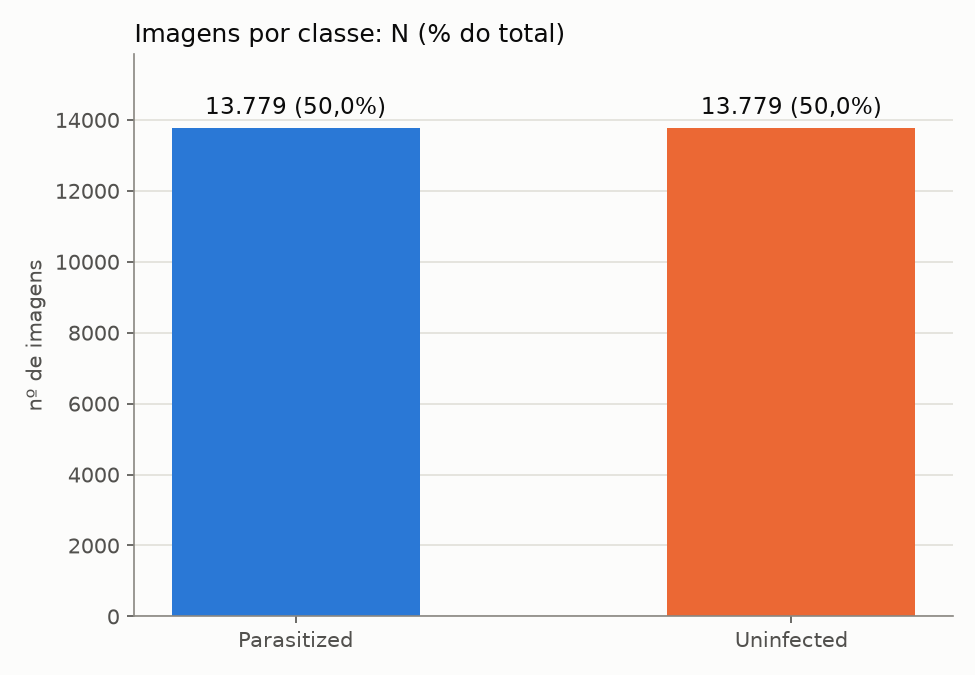
\includegraphics[width=0.55\textwidth]{balanceamento_classes.png}
\caption{Número de imagens válidas por classe, com a porcentagem do total.
Arquivo: \texttt{balanceamento\_classes.png}.}\label{fig:balanceamento}
\end{figure}

\subsection{Modo de cor e dimensões}

Todas as 27.558 imagens estão no modo RGB (3 canais de 8 bits). Por isso a conversão de modo de cor
(\texttt{convert("RGB")}) foi removida do pipeline: ela não alterava nenhuma imagem.

As dimensões, por outro lado, variam bastante (Figura~\ref{fig:dimensoes}): há 1.627 tamanhos
distintos, de $46\times40$ até $394\times385$ pixels, com mediana de $130\times130$. Apenas 7,9\% das
imagens são quadradas; a razão largura/altura vai de 0,46 a 2,59. Como cada recorte envolve uma
única hemácia, a dimensão da imagem acompanha o diâmetro da célula. As medianas das duas classes são
próximas (133 px nas parasitadas e 130 px nas não infectadas).

Um detalhe observado: larguras e alturas só ocorrem de 3 em 3 pixels (112, 115, 118\ldots), e as
bordas dos recortes têm degraus de cerca de 3 px (visíveis na Figura~\ref{fig:exemplos}). Isso
sugere que os autores ampliaram a máscara de segmentação por um fator 3 ao gerar os recortes. Para os
histogramas da Figura~\ref{fig:dimensoes}, a largura das faixas foi escolhida como múltiplo desse
passo (6 px); com faixas de 5 px, umas faixas recebiam um valor possível e outras dois, e o
histograma ficava serrilhado.

\begin{figure}[H]
\centering
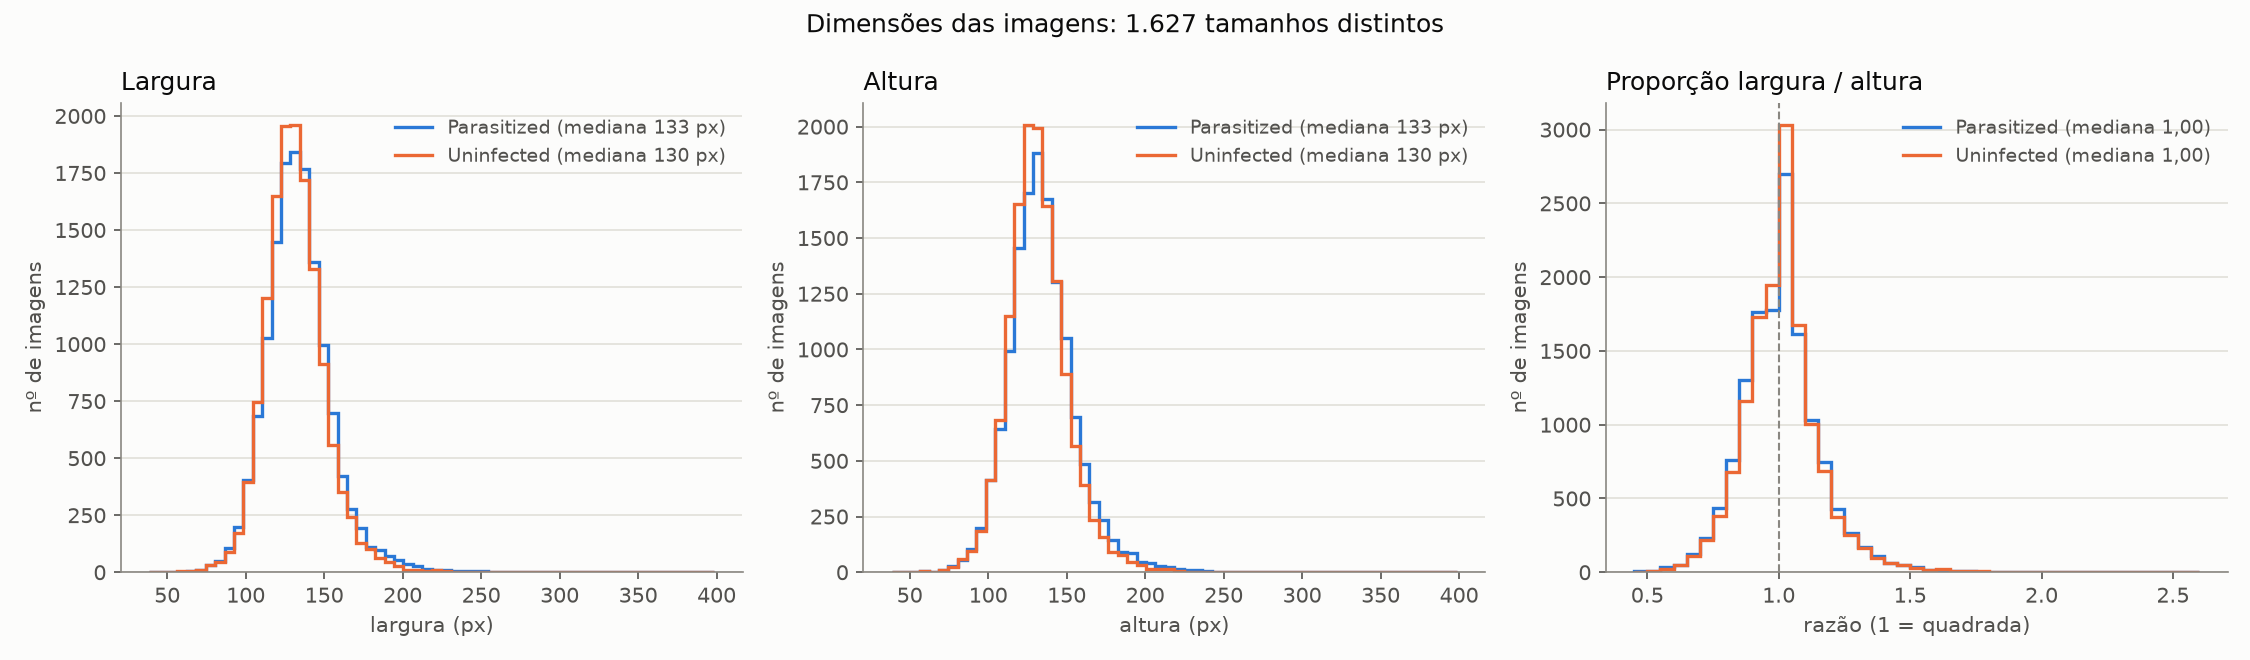
\includegraphics[width=\textwidth]{dimensoes_imagens.png}
\caption{Distribuição da largura, da altura e da proporção largura/altura das imagens originais,
por classe. A linha tracejada marca a proporção 1 (imagem quadrada).
Arquivo: \texttt{dimensoes\_imagens.png}.}\label{fig:dimensoes}
\end{figure}

\subsection{Exemplos e dificuldades do problema}

A Figura~\ref{fig:exemplos} mostra imagens sorteadas de cada classe. Elas evidenciam as principais
dificuldades do problema:
\begin{itemize}
  \item \textbf{Variação de coloração entre lâminas.} A cor de fundo da célula vai do rosa ao lilás e
        ao azul-acinzentado nas duas classes. Essa variação vem do corante, da espessura do
        esfregaço e da iluminação de cada lâmina, e não da infecção. Para um classificador baseado em
        cor, ela é ruído --- e um ruído correlacionado com o paciente.
  \item \textbf{Parasitas pequenos ou pouco corados.} Em várias células parasitadas o parasita é
        um ponto roxo de poucos pixels, às vezes na borda da célula.
  \item \textbf{Artefatos nas não infectadas.} Algumas células não infectadas têm manchas, regiões
        claras no centro (palidez central da hemácia) ou plaquetas sobrepostas, que podem ser
        confundidas com o parasita.
  \item \textbf{Recortes imperfeitos.} Há recortes com parte de uma célula vizinha ou com a célula
        cortada, herdados da segmentação automática feita pelos autores.
\end{itemize}

\begin{figure}[H]
\centering
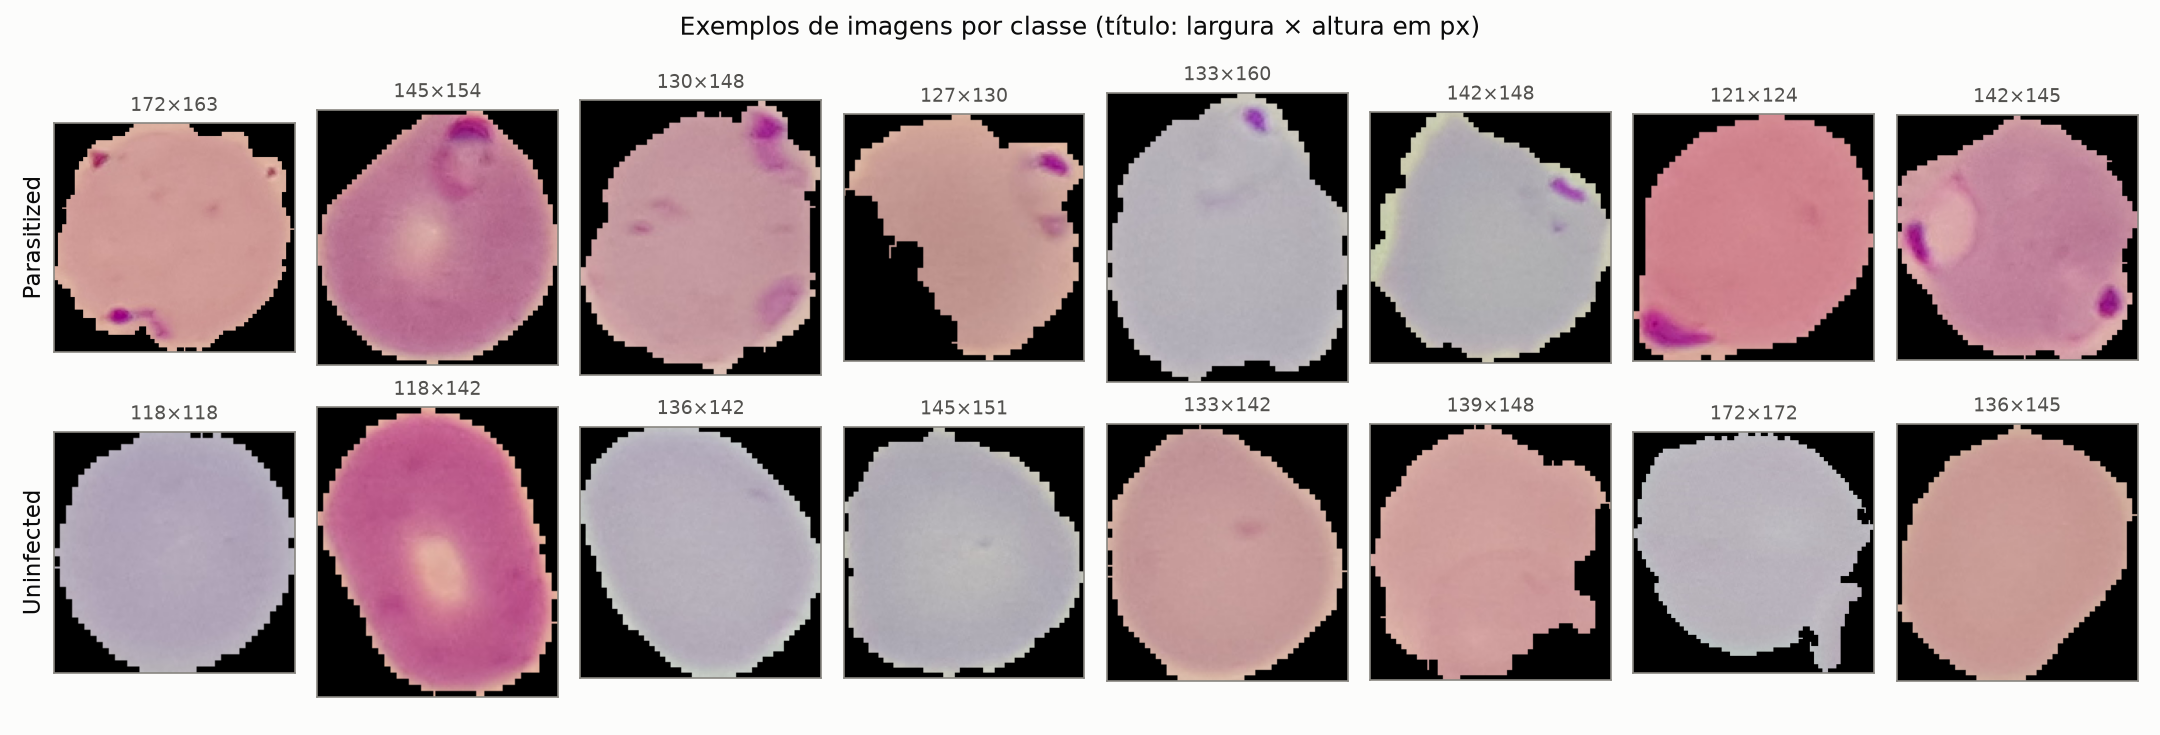
\includegraphics[width=\textwidth]{exemplos_imagens.png}
\caption{Oito imagens sorteadas de cada classe (semente 42). O título de cada imagem indica suas
dimensões originais. Arquivo: \texttt{exemplos\_imagens.png}.}\label{fig:exemplos}
\end{figure}

\subsection{Análise de cor}\label{sec:cor}

Como a diferença entre as classes é essencialmente de cor (o parasita corado em roxo dentro de uma
célula rosada), a distribuição de cores foi analisada considerando apenas os pixels da célula, isto é,
excluindo o fundo preto $(0,0,0)$. Todas as imagens válidas foram usadas.

\paragraph{Histograma por canal.} A Figura~\ref{fig:canais} mostra a distribuição de intensidade de
cada canal R, G e B, normalizada pelo total de pixels de célula de cada classe. O eixo vertical está
em escala logarítmica porque os pixels do parasita são poucos: na escala linear a diferença entre as
classes desaparece. O canal verde (G) é o que mais separa as classes: as células parasitadas têm uma
cauda longa de pixels escuros em G (intensidade abaixo de $\sim$130), dezenas de vezes mais frequente
que nas não infectadas. Isso tem explicação física: o corante Giemsa deixa a cromatina do parasita
roxa, e o roxo absorve o verde. No canal B há uma cauda semelhante, mais fraca; no canal R as
classes são quase idênticas.

\begin{figure}[H]
\centering
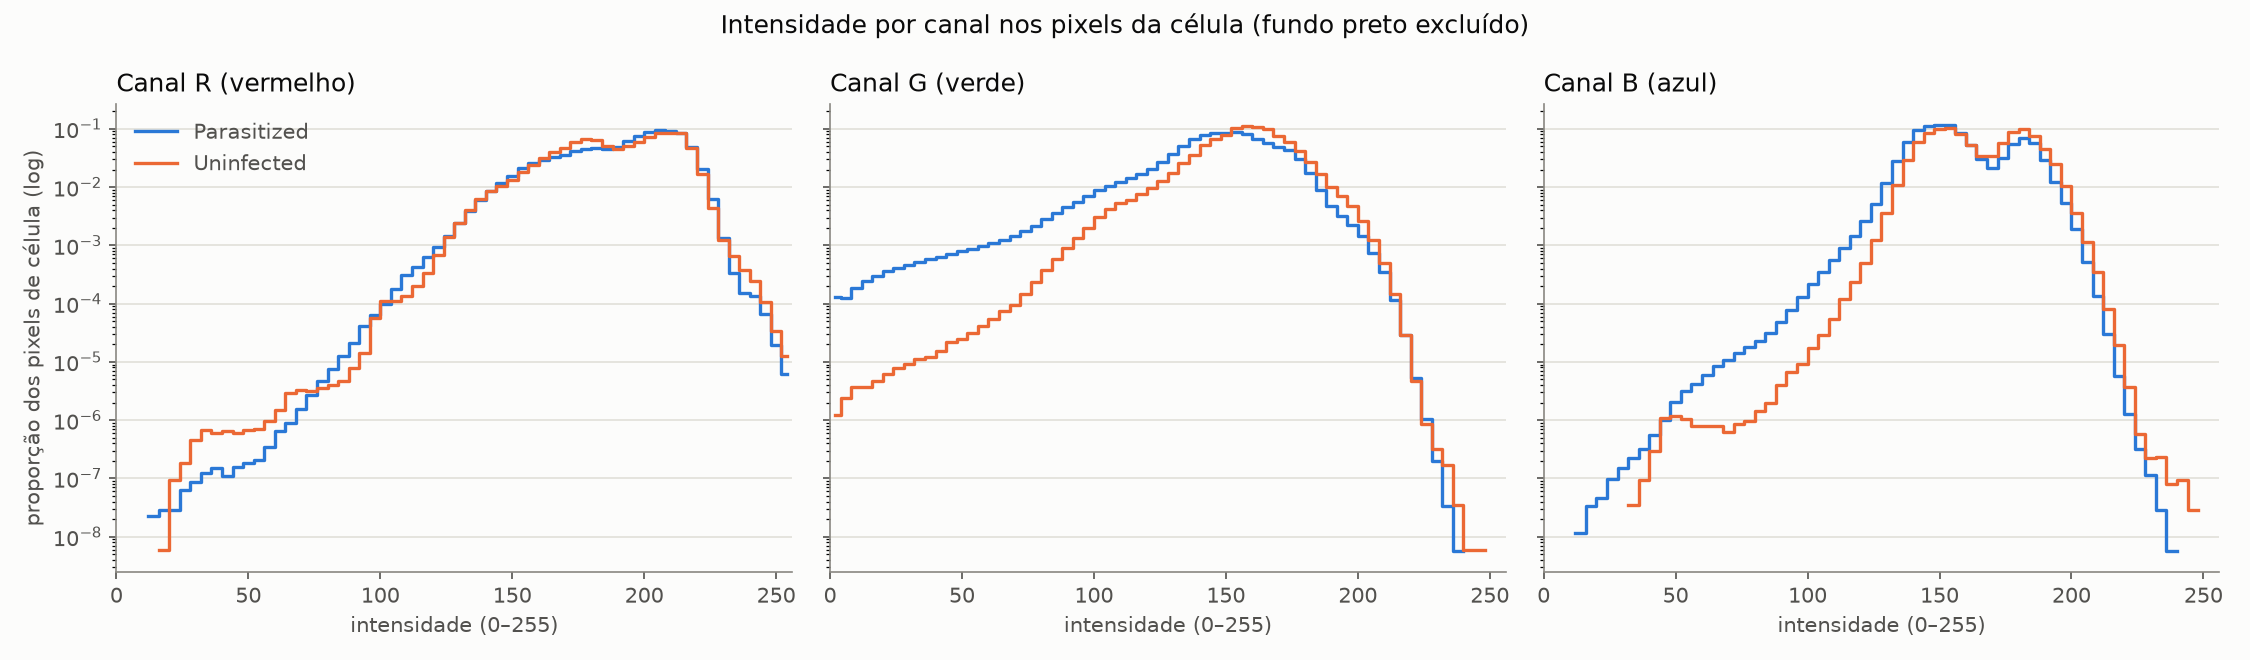
\includegraphics[width=\textwidth]{histograma_canais_rgb.png}
\caption{Intensidade de cada canal RGB nos pixels da célula (fundo excluído), por classe, em escala
logarítmica. Arquivo: \texttt{histograma\_canais\_rgb.png}.}\label{fig:canais}
\end{figure}

\paragraph{Paleta de cores.} Para ver quais cores aparecem nas imagens, cada canal foi quantizado em
8 níveis (faixas de 32 tons), o que resulta em até $8^3=512$ cores. Para cada cor quantizada foram
calculados a cor média real dos pixels que caem nela, a proporção dos pixels de célula de cada
classe que ela ocupa e a razão entre a proporção numa classe e a proporção na outra. A
Figura~\ref{fig:paleta} mostra, para cada classe, as 12 cores mais frequentes (à esquerda) e as 12
cores mais típicas da classe, isto é, com maior razão (à direita; só cores com pelo menos 0,02\% dos
pixels da classe). A tabela completa está em \arq{outputs/cores_quantizadas.csv}.

\begin{figure}[H]
\centering
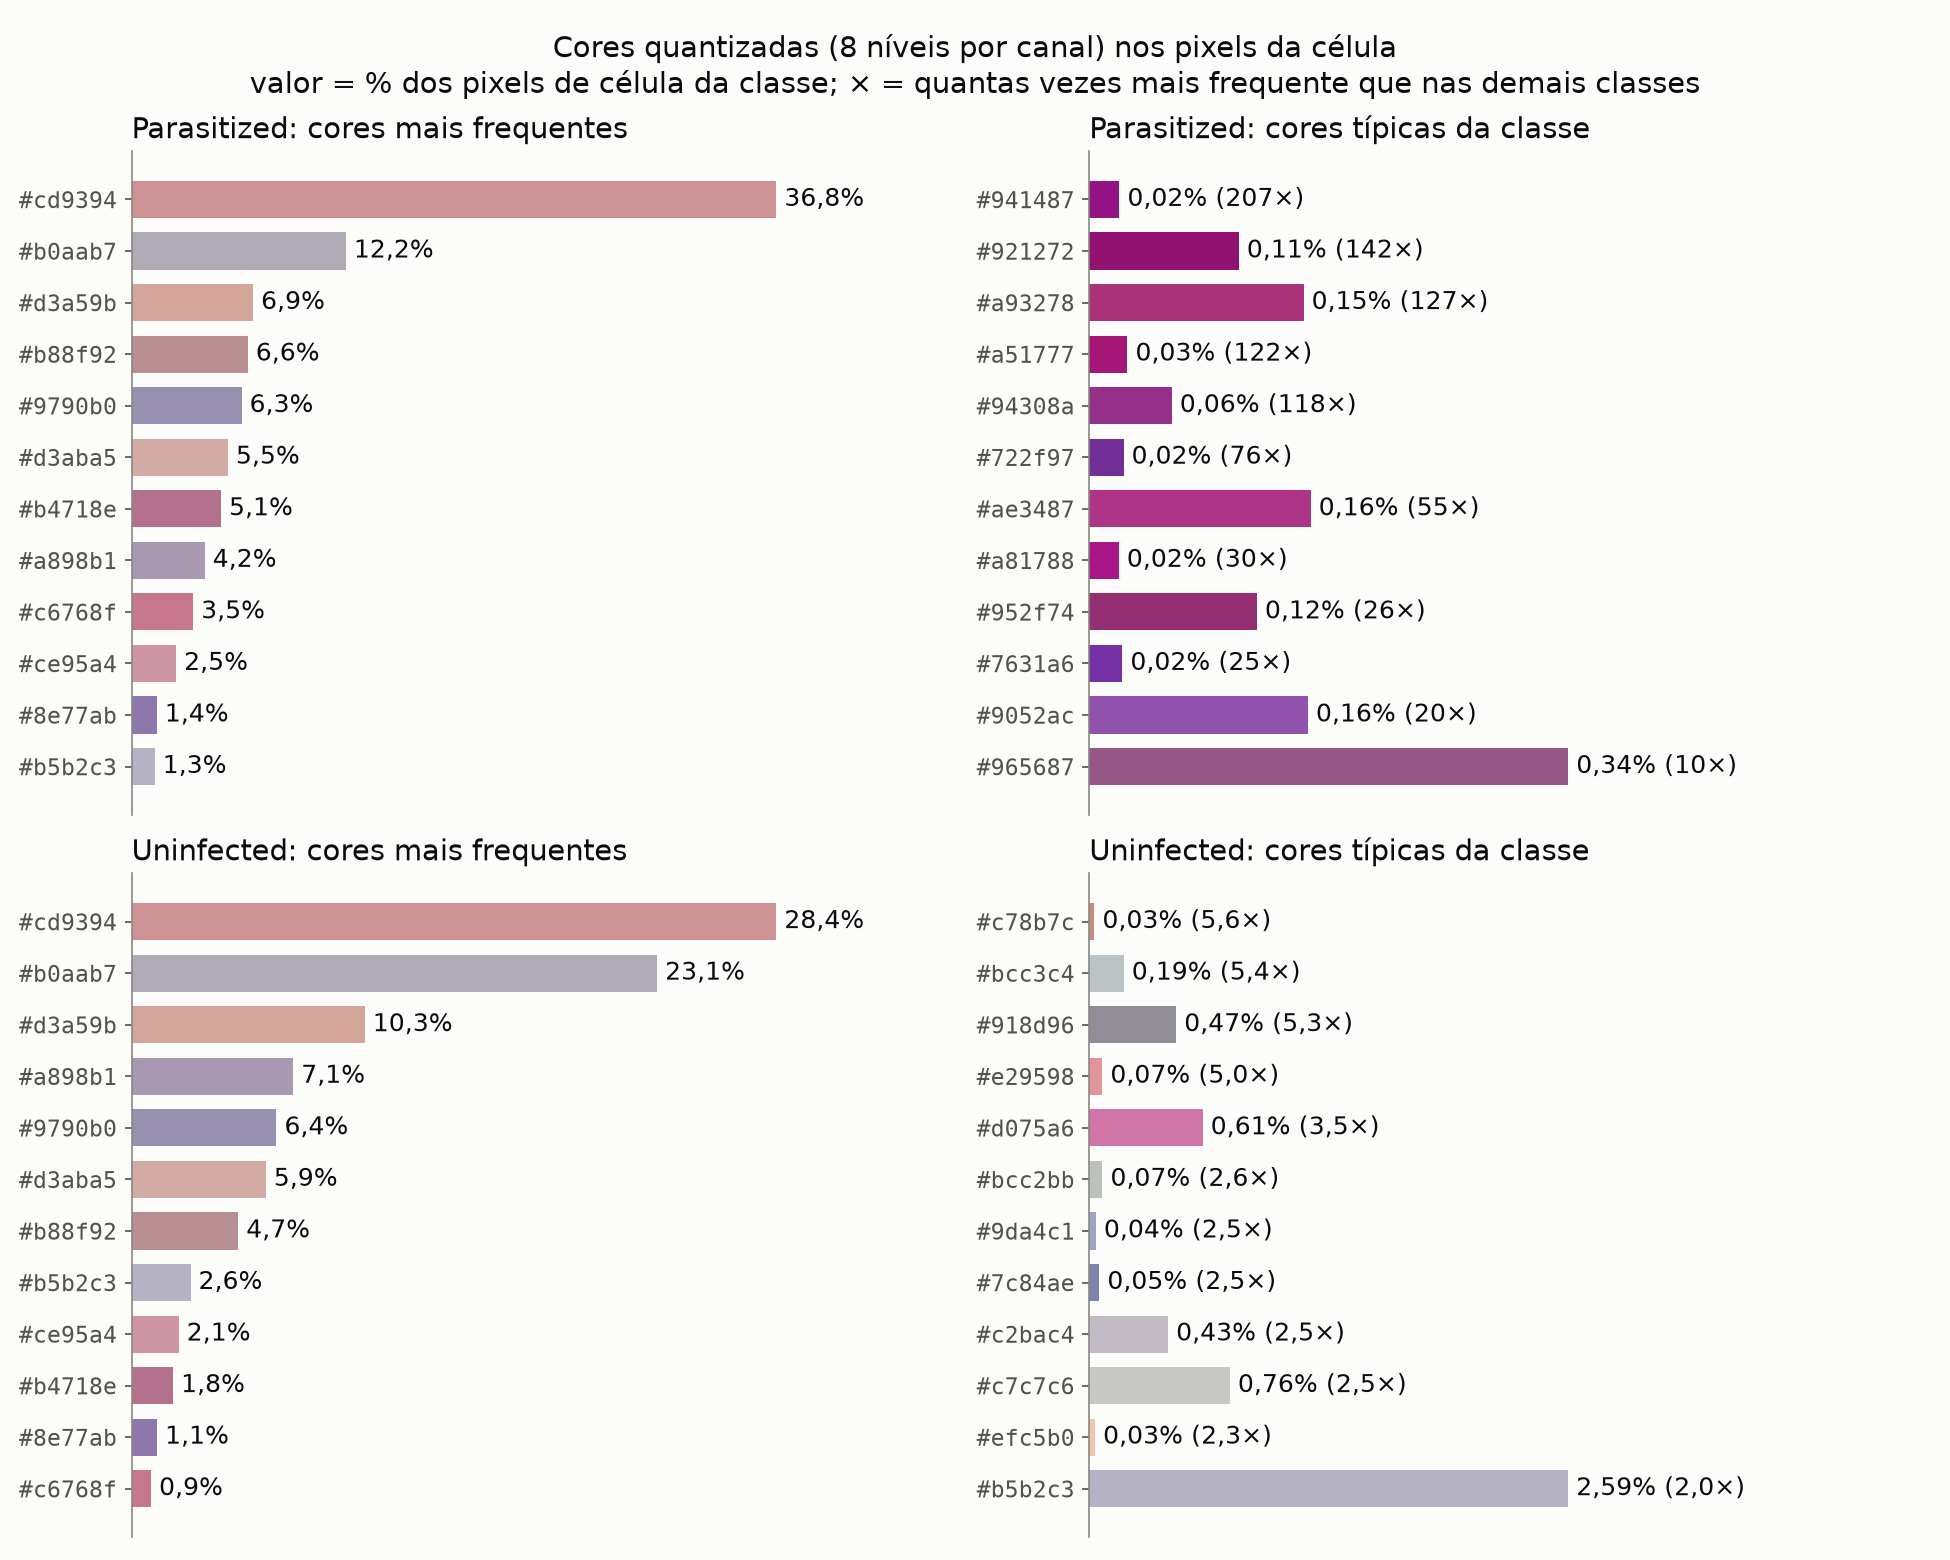
\includegraphics[width=\textwidth]{paleta_cores.png}
\caption{Cores quantizadas (8 níveis por canal) nos pixels da célula. Cada barra é pintada com a
própria cor. Valor: \% dos pixels de célula da classe; ``$\times$'': quantas vezes a cor é mais
frequente nesta classe do que na outra. Arquivo: \texttt{paleta\_cores.png}.}\label{fig:paleta}
\end{figure}

Conclusões da análise de cor:
\begin{itemize}
  \item As cores \emph{mais frequentes} são as mesmas nas duas classes (rosa \texttt{\#cd9394},
        lilás \texttt{\#b0aab7} etc.). Ou seja, a cor média da célula diz pouco sobre a classe e
        reflete principalmente a coloração da lâmina.
  \item As cores \emph{típicas} das parasitadas são roxos e magentas escuros (por exemplo
        \texttt{\#941487}, 207 vezes mais frequente que nas não infectadas). Cada uma ocupa menos
        de 0,5\% dos pixels, mas elas são quase exclusivas dessa classe: é o parasita.
  \item As cores típicas das não infectadas têm razões baixas (no máximo 5,6 vezes) e são tons
        acinzentados, ou seja, não existe uma cor exclusiva da célula sadia.
\end{itemize}

Essas observações orientaram três decisões: usar características de \emph{distribuição} de cor
(histogramas e desvios), e não só médias; considerar a cauda escura do canal G; e testar uma
normalização que remova a coloração da lâmina (Seção~\ref{sec:normalizacao}).

%=====================================================================
\section{Divisão em treino e teste}\label{sec:divisao}
%=====================================================================

As células de um mesmo paciente compartilham a coloração da lâmina, a iluminação e o estágio da
infecção. Se células do mesmo paciente aparecessem no treino e no teste, o classificador poderia
acertar no teste por reconhecer a lâmina, e não o parasita, e o desempenho medido seria otimista. Por
isso, conforme exigido no enunciado, todas as imagens de um paciente ficam no mesmo conjunto.

A divisão usa \texttt{StratifiedGroupKFold} (scikit-learn~\cite{sklearn}) com 5 partições,
embaralhamento e semente 42, com o paciente como grupo e a classe como estratificação. A primeira
partição é o conjunto de teste (cerca de 20\% dos pacientes) e as outras quatro formam o treino. A
estratificação mantém a proporção das classes parecida nos dois conjuntos, apesar de as células
virem em blocos por paciente. A divisão é idêntica em todas as configurações comparadas.

\begin{table}[H]
\centering
\caption{Divisão treino/teste por paciente. Nenhum paciente aparece nos dois conjuntos.}\label{tab:divisao}
\begin{tabular}{lrrrr}
\toprule
Conjunto & Parasitized & Uninfected & Total & Pacientes \\
\midrule
Treino & 10.975 & 11.028 & 22.003 & 160 \\
Teste  &  2.804 &  2.751 &  5.555 &  40 \\
\midrule
Total  & 13.779 & 13.779 & 27.558 & 200 \\
\bottomrule
\end{tabular}
\par\vspace{2pt}\footnotesize Fonte: saída do console de \arq{2_classificacao.py} (função \texttt{describe\_split}).
\end{table}

O conjunto de teste foi usado \emph{uma única vez} por configuração, para a avaliação final. Toda a
seleção de hiperparâmetros e todas as escolhas entre configurações foram feitas com validação
cruzada dentro do treino (Seção~\ref{sec:classificacao}), também agrupada por paciente.

%=====================================================================
\section{Pré-processamento}\label{sec:preproc}
%=====================================================================

O pré-processamento de cada imagem é feito na função \texttt{extract} de
\arq{2_classificacao.py}, nesta ordem: leitura, redimensionamento, mudança de escala para $[0,1]$,
segmentação (Seção~\ref{sec:segmentacao}), normalização de cor (opcional) e conversões de espaço de
cor. Cada operação tem uma finalidade ligada a uma característica observada do dataset.

\subsection{Leitura e escala de intensidade}

A imagem é lida diretamente, sem conversão de modo de cor, pois todas já são RGB. Os valores são
convertidos para ponto flutuante e divididos por 255, ficando em $[0,1]$. Essa escala é a esperada
pelas conversões de cor do scikit-image~\cite{skimage} e pelos histogramas, que usam faixas fixas no
intervalo $[0,1]$.

\subsection{Redimensionamento}\label{sec:resize}

Como as imagens têm tamanhos diferentes (Figura~\ref{fig:dimensoes}), foi preciso decidir como
tratá-las. Três opções foram implementadas e comparadas experimentalmente
(Seção~\ref{sec:res-preproc}):
\begin{itemize}
  \item \textbf{64x64}: todas as imagens são redimensionadas para $64\times64$ com interpolação
        bilinear. É a opção mais rápida, mas cada imagem é reduzida por um fator diferente (a de 394
        px é reduzida cerca de 6 vezes; a de 46 px é ampliada) e a proporção da célula é distorcida.
  \item \textbf{fator2}: todas as imagens são reduzidas à metade do próprio tamanho
        (\texttt{Image.reduce(2)}, média de blocos $2\times2$). Como todas as células foram fotografadas
        com a mesma ampliação, um pixel continua representando o mesmo tamanho físico em todas, e a
        proporção é preservada.
  \item \textbf{original}: sem redimensionamento. Preserva todo o detalhe, ao custo de uma extração
        cerca de duas vezes mais lenta.
\end{itemize}

Nenhuma das características extraídas exige tamanho fixo: todas são estatísticas ou histogramas
normalizados pelo número de pixels da célula (Seção~\ref{sec:features}). Por isso as três opções
são possíveis. O redimensionamento tem dois efeitos: reduz o custo de processamento e altera a escala
em que a textura é medida pelo LBP.

Nos experimentos, as três opções empataram na validação cruzada (diferença inferior a 0,002 no F1
macro, contra um desvio de $\sim$0,01 entre as partições). Como a mudança não teve efeito mensurável,
a configuração final manteve o \textbf{64x64}, a opção mais simples e rápida.

\subsection{Normalização de cor}\label{sec:normalizacao}

A análise de cor (Seção~\ref{sec:cor}) mostrou que a coloração geral da célula muda de lâmina para
lâmina e não depende da classe. Para remover esse efeito foi usada a hipótese do \emph{mundo
cinza}~\cite{buchsbaum1980}, aplicada só dentro da célula: cada canal $c\in\{R,G,B\}$ é multiplicado
por um fator que leva a média dos pixels da célula a um cinza neutro fixo:
\begin{equation}
  I'_c(x,y) = \min\!\left(1,\; I_c(x,y)\cdot\frac{0{,}6}{\mu_c}\right),
  \qquad \mu_c = \frac{1}{|M|}\sum_{(x,y)\in M} I_c(x,y),
\end{equation}
em que $M$ é o conjunto de pixels da máscara da célula. Depois disso, todas as células têm a mesma
cor média; o que sobra é a variação \emph{dentro} da célula. Como o parasita ocupa poucos pixels, ele
quase não altera a média e continua mais escuro e roxo que o restante da célula (última coluna da
Figura~\ref{fig:segmentacao}).

Duas variantes foram consideradas e descartadas:
\begin{itemize}
  \item \emph{Normalização por classe}: usaria o rótulo, que é desconhecido no momento da previsão,
        e portanto vazaria a resposta.
  \item \emph{Normalização de Reinhard} (igualar média \emph{e desvio} de cada canal no espaço Lab):
        igualar o desvio aumentaria o contraste das células sadias (desvio pequeno) e reduziria o das
        parasitadas (desvio grande), apagando justamente a diferença que interessa.
\end{itemize}
A normalização usa apenas a própria imagem; nenhum parâmetro é aprendido dos dados.

\subsection{Conversões de espaço de cor}

Duas conversões são feitas após a normalização:
\begin{itemize}
  \item \textbf{Tons de cinza} (\texttt{rgb2gray}, $Y = 0{,}2125R + 0{,}7154G + 0{,}0721B$): entrada do
        descritor de textura LBP.
  \item \textbf{HSV} (\texttt{rgb2hsv}): separa matiz (H), saturação (S) e brilho (V). A saturação é
        útil porque o parasita é muito mais saturado que o citoplasma; o matiz exige tratamento
        especial (Seção~\ref{sec:matiz}).
\end{itemize}

%=====================================================================
\section{Segmentação}\label{sec:segmentacao}
%=====================================================================

\subsection{Por que segmentar}

Em média, cerca de 30\% dos pixels de cada imagem são fundo preto. Esse fundo é igual nas duas classes e
não carrega informação, mas, se entrasse nas estatísticas, mudaria a média, o desvio e os histogramas
de acordo com o formato e o tamanho do recorte, e não de acordo com o conteúdo da célula. Por isso
todas as características são calculadas só sobre os pixels da célula. A contribuição da segmentação
foi medida diretamente (Seção~\ref{sec:res-seg}).

\subsection{Método}

O dataset já vem com a célula separada do fundo pelos autores, e o fundo é \emph{exatamente}
$(0,0,0)$. A segmentação, portanto, é uma limiarização com limiar zero, seguida de uma operação
morfológica:
\begin{enumerate}
  \item \textbf{Máscara na resolução original}: $M(x,y)=1$ se $\max(R,G,B)>0$. Numa amostra de 300
        imagens originais, o fundo vale exatamente 0 e nenhum pixel de célula tem cinza abaixo de
        0,1, então a separação é exata.
  \item \textbf{Redimensionamento da máscara} para o tamanho da imagem processada, com interpolação
        pelo vizinho mais próximo (\texttt{NEAREST}), que não cria valores intermediários.
  \item \textbf{Erosão} com elemento estruturante em disco de raio 1 (cruz $3\times3$). O
        redimensionamento bilinear mistura fundo e célula na borda; a erosão descarta esse anel de
        pixels misturados.
\end{enumerate}

\paragraph{Versão anterior e correção.} A primeira versão calculava a máscara \emph{depois} do
redimensionamento, com um limiar fixo de 0,04 no tom de cinza. Medindo a distribuição de cinza em 300
imagens, verificou-se que o redimensionamento bilinear cria pixels de borda com valores entre 0 e 0,4,
e cerca de 4\% dos pixels contados como célula eram, na verdade, mistura de célula com fundo: o
percentil 1 do cinza da célula caía de 0,415 (imagem original) para 0,09. Com a máscara calculada na
resolução original, redimensionada por vizinho mais próximo e erodida, o percentil 1 voltou a 0,405.
Simplesmente aumentar o limiar não resolveria, porque os pixels mais escuros da célula (cinza entre 0,1
e 0,4) são justamente os do parasita.

\begin{figure}[H]
\centering
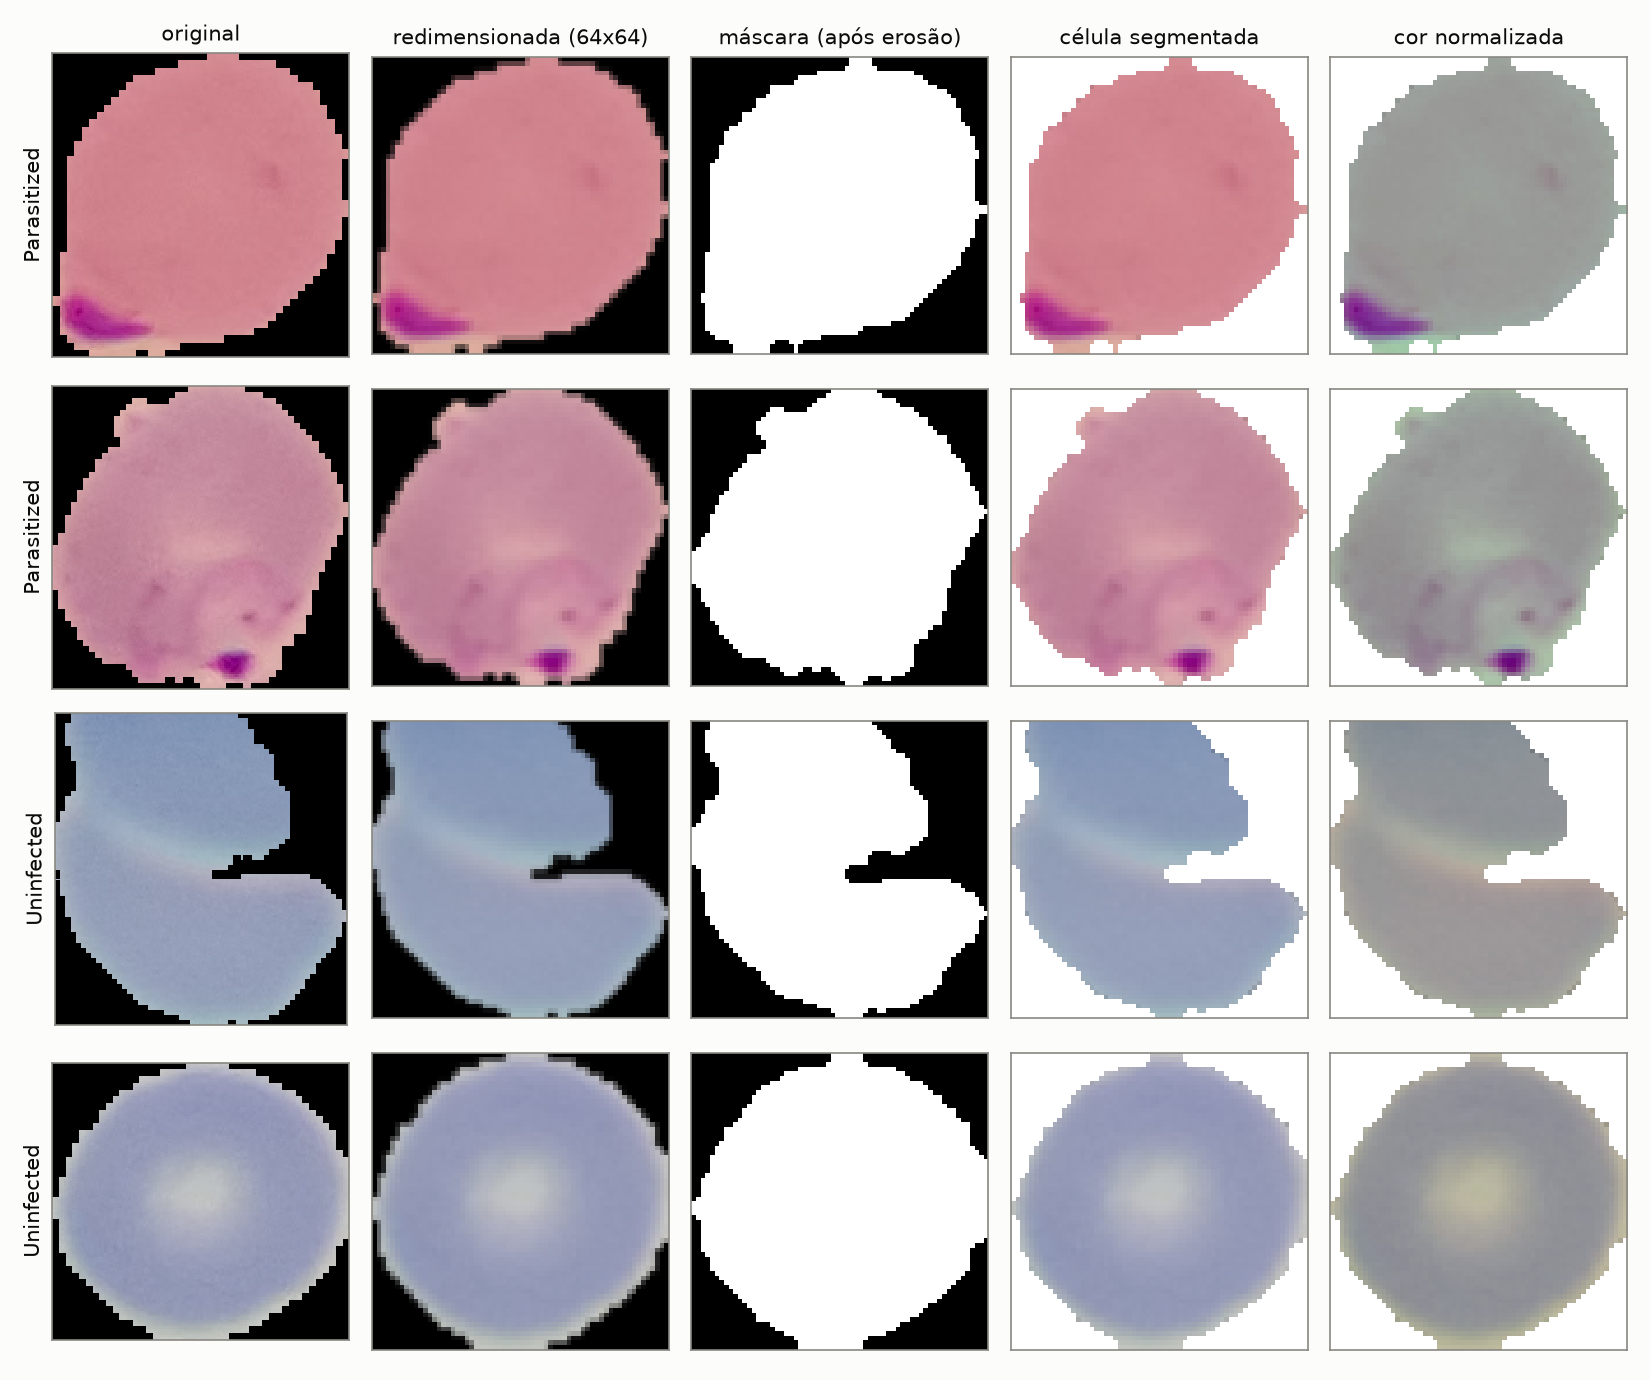
\includegraphics[width=\textwidth]{exemplos_segmentacao.png}
\caption{Etapas do pré-processamento em quatro células sorteadas: imagem original, imagem
redimensionada para $64\times64$, máscara após a erosão, célula segmentada (fundo descartado
em branco) e cor normalizada. Arquivo: \texttt{exemplos\_segmentacao.png}.}\label{fig:segmentacao}
\end{figure}

\subsection{Limitações}

\begin{itemize}
  \item A segmentação herda os defeitos da segmentação original dos autores: recortes com parte de
        uma célula vizinha (terceira linha da Figura~\ref{fig:segmentacao}) ou com bordas em degrau.
  \item A erosão remove uma faixa de 1 pixel da borda. Parasitas encostados na membrana da célula
        perdem parte dos seus pixels.
  \item O descritor LBP compara cada pixel com seus 8 vizinhos. Perto da borda, alguns desses
        vizinhos ainda são pixels misturados com o fundo, o que gera padrões de ``borda'' que não são
        textura da célula.
\end{itemize}

%=====================================================================
\section{Extração de características e dataframe}\label{sec:features}
%=====================================================================

\subsection{Características}

Para cada imagem são extraídas 71 características, todas calculadas apenas sobre os pixels da
máscara $M$ e, quando são contagens, divididas por $|M|$. Isso as torna independentes do tamanho da
imagem.

\begin{table}[H]
\centering
\caption{Características extraídas por imagem.}\label{tab:features}
\begin{tabular}{lp{7.2cm}rl}
\toprule
Grupo & Características & Qtd. & Referência \\
\midrule
Cor -- momentos RGB & média e desvio de R, G, B & 6 & \cite{stricker1995} \\
Cor -- momentos HSV & média e desvio de S e V & 4 & \cite{stricker1995} \\
Cor -- matiz (circular) & 1º momento trigonométrico $(C,S)$ e desvio circular de H & 3 & \cite{mardia2000} \\
Cor -- histogramas & histograma de R, G e B, 16 faixas cada, normalizado & 48 & \cite{swain1991} \\
Textura -- LBP & histograma LBP$^{riu2}_{8,1}$ (10 padrões), normalizado & 10 & \cite{ojala2002} \\
\midrule
Total & & 71 & \\
\bottomrule
\end{tabular}
\end{table}

\paragraph{Momentos de cor.} Média e desvio padrão de cada canal resumem a distribuição de cor da
célula com poucos números~\cite{stricker1995}. O desvio é especialmente útil aqui: uma célula
parasitada tem pixels muito diferentes entre si (citoplasma claro e parasita escuro), então seu desvio
é maior.

\paragraph{Matiz como variável circular.}\label{sec:matiz} O matiz H é um ângulo: os valores 0 e 1
representam o mesmo vermelho. O rosa das hemácias fica justamente nessa virada (H entre $\sim$0,97 e
$\sim$0,03). Na primeira versão, o matiz era tratado como uma variável linear e a média aritmética de
uma célula com pixels nos dois lados da virada dava $\sim$0,5 (ciano), uma cor que não existe na
célula. Isso foi detectado na verificação das características: entre os percentis 5 e 95, a média
do matiz ia de 0,02 a 0,94, e o desvio chegava a 0,496, quase o máximo possível em $[0,1]$ --- efeito
da virada, não variação real de cor. A correção usa estatística circular~\cite{mardia2000}, com cada pixel ponderado pela
saturação, porque o matiz de um pixel quase cinza é instável:
\begin{equation}
  C = \frac{\sum_i s_i \cos\theta_i}{\sum_i s_i},\qquad
  S = \frac{\sum_i s_i \sin\theta_i}{\sum_i s_i},\qquad
  R = \sqrt{C^2+S^2},\qquad
  \sigma_{\text{circ}} = \sqrt{-2\ln R},
\end{equation}
em que $\theta_i = 2\pi H_i$ e $s_i$ é a saturação do pixel $i$. O par $(C,S)$ é o primeiro momento
trigonométrico (a média circular): sua direção é o matiz médio e seu comprimento $R$ mede o quanto os
matizes estão concentrados. As características são $C$, $S$ e $\sigma_{\text{circ}}$. Usar os
componentes $(C,S)$, e não o ângulo, evita reintroduzir o salto entre 0 e 1 e mantém os valores
estáveis quando $R\approx0$, o que acontece após a normalização de cor (célula quase cinza).

\paragraph{Histogramas de cor.} Cada canal é dividido em 16 faixas de mesma largura no intervalo
$[0,1]$, e a contagem de cada faixa é dividida pelo número de pixels da célula~\cite{swain1991}. Os
histogramas capturam a cauda escura do parasita, que a média e o desvio resumem mal
(Figura~\ref{fig:canais}).

\paragraph{Textura (LBP).} O \emph{Local Binary Pattern} compara cada pixel $g_c$ com $P$ vizinhos
$g_p$ num círculo de raio $R$ e forma um código binário. Foi usada a variante invariante à rotação e
uniforme (riu2) de Ojala et al.~\cite{ojala2002}, com $P=8$ e $R=1$:
\begin{equation}
  \mathrm{LBP}^{riu2}_{P,R} =
  \begin{cases}
    \sum_{p=0}^{P-1} s(g_p - g_c) & \text{se } U \le 2,\\
    P+1 & \text{caso contrário,}
  \end{cases}
  \qquad s(x)=\begin{cases}1 & x\ge 0\\ 0 & x<0\end{cases}
\end{equation}
em que $U$ é o número de transições 0/1 no código circular. Há $P+2=10$ valores possíveis, e o
histograma desses valores, normalizado, é o descritor. A invariância à rotação é adequada porque a
célula pode aparecer em qualquer orientação. O LBP é calculado na imagem em tons de cinza inteira e
só os pixels da máscara entram no histograma.

\paragraph{Verificação das características.} Antes da versão final, as características foram
analisadas no conjunto de treino quanto a redundância e poder de separação. Os principais achados:
\begin{itemize}
  \item cerca de 15 das 48 faixas de histograma são quase sempre zero (faixas extremas, onde não
        existe pixel de célula) e, em cada histograma, as faixas somam 1, o que cria dependências
        lineares exatas. Isso não prejudica os modelos (a regressão logística é regularizada e o SVM é
        robusto a dimensões constantes), mas indica redundância;
  \item a característica isolada mais discriminante foi uma faixa intermediária do histograma do canal
        G (AUC de 0,95), coerente com a análise de cor;
  \item o problema do matiz descrito acima, que foi corrigido.
\end{itemize}
A comparação entre conjuntos de características (só cor vs. cor + textura) está na
Seção~\ref{sec:res-features}.

\subsection{Dataframe}

As características de todas as imagens formam um dataframe com uma linha por imagem e as colunas:
\texttt{id} (nome do arquivo, único em todo o dataset), \texttt{classe}, \texttt{paciente} e as 71
características. O \texttt{id} e o \texttt{paciente} não entram no classificador: o paciente é usado
apenas para formar os grupos na divisão treino/teste e na validação cruzada. O dataframe de cada
configuração é salvo em \arq{outputs/<config>/features_<config>.csv}; o da configuração
final é \arq{outputs/64x64_normalizacao_cor/features_64x64_normalizacao_cor.csv}.

%=====================================================================
\section{Classificação e protocolo de avaliação}\label{sec:classificacao}
%=====================================================================

\subsection{Modelos}

\begin{itemize}
  \item \textbf{Baseline}: \texttt{DummyClassifier} que sempre prevê a classe mais frequente do treino
        (Uninfected, com 11.028 contra 10.975). Serve de referência mínima.
  \item \textbf{SVM com kernel RBF} (\texttt{SVC}): modelo não linear de margem máxima. Hiperparâmetros:
        $C$ (penalidade de erro) e $\gamma$ (alcance do kernel).
  \item \textbf{Regressão logística} (\texttt{LogisticRegression}, regularização L2): modelo linear,
        rápido e interpretável. Hiperparâmetro: $C$ (inverso da regularização).
\end{itemize}

Cada modelo é um \texttt{Pipeline} com \texttt{StandardScaler} seguido do classificador. A
padronização é necessária para os dois modelos (o kernel RBF depende de distâncias e a regularização
da regressão logística depende da escala) e, por estar dentro do pipeline, é ajustada só com os dados
de treino de cada partição, sem vazamento.

\subsection{Seleção de hiperparâmetros}

A busca é feita com \texttt{GridSearchCV} no conjunto de treino, com validação cruzada
\texttt{StratifiedGroupKFold} de 5 partições agrupadas por paciente e F1 macro como critério. As
grades são:
\begin{itemize}
  \item SVM: $C\in\{1, 10, 100, 1000\}$ e $\gamma\in\{10^{-4}, 10^{-3}, 10^{-2}\}$ (12 combinações);
  \item Regressão logística: $C\in\{10^{-4}, 10^{-3},\ldots,10^{2}\}$ (7 valores).
\end{itemize}

A grade do SVM foi ajustada durante o trabalho. A grade inicial era $C\in\{0{,}1;\,1;\,10;\,100\}$ e
$\gamma\in\{10^{-3},10^{-2},10^{-1}\}$, e o melhor ponto ficou no canto $C=100$, $\gamma=10^{-3}$. Os
resultados mostraram que os melhores pontos ficam numa diagonal ($C\cdot\gamma\approx0{,}1$) e que
$C=0{,}1$ e $\gamma=0{,}1$ estavam sempre entre os piores. A grade foi então deslocada nessa direção.
Na configuração final o ótimo ($C=100$, $\gamma=10^{-3}$) fica no interior da grade, e os cinco
melhores pontos estão a menos de 0,001 de F1 um do outro (Tabela~\ref{tab:grid-svm}), ou seja, o
desempenho é estável em relação aos hiperparâmetros.

\subsection{Métricas e procedimento}

Para cada modelo:
\begin{enumerate}
  \item a busca escolhe os hiperparâmetros pelo F1 macro médio da validação cruzada;
  \item com esses hiperparâmetros, \texttt{cross\_val\_predict} gera uma predição \emph{fora da
        partição} (out-of-fold) para cada imagem do treino, nas mesmas partições. As métricas de
        validação cruzada são calculadas sobre essas predições;
  \item o modelo é reajustado em todo o treino e avaliado uma vez no conjunto de teste.
\end{enumerate}
As métricas reportadas são acurácia, precisão, recall e F1 por classe, F1 macro (média simples do F1
das duas classes) e matriz de confusão. Os resultados de cada configuração ficam em
\arq{outputs/<config>/validacao_cruzada/} e \arq{outputs/<config>/testset/}.

%=====================================================================
\section{Resultados}\label{sec:resultados}
%=====================================================================

\subsection{Evolução do pipeline}\label{sec:evolucao}

A Tabela~\ref{tab:evolucao} resume como cada decisão alterou o desempenho do SVM, na ordem em que foram
tomadas. As linhas 2 e 3 são de execuções intermediárias cujas saídas foram substituídas pelas
seguintes; os números foram registrados durante o desenvolvimento.

\begin{table}[H]
\centering
\caption{Evolução do F1 macro do SVM a cada decisão do pipeline.}\label{tab:evolucao}
\begin{tabular}{cp{8.6cm}cc}
\toprule
\# & Mudança & F1 macro CV & F1 macro teste \\
\midrule
1 & Versão inicial (máscara com limiar 0,04 após o resize, 64x64) & 0,922 & 0,929 \\
2 & Máscara na resolução original + erosão & 0,931 & 0,930 \\
3 & + normalização de cor por imagem & 0,954 & 0,956 \\
4 & + matiz circular e grade do SVM ajustada & 0,954 & 0,955 \\
5 & Redimensionamento fator2 ou original (descartado) & 0,955 & 0,959 / 0,961 \\
\bottomrule
\end{tabular}
\par\vspace{2pt}\footnotesize Fonte: linha 1, \arq{outputs/validacao_cruzada/} e \arq{outputs/testset/};
linha 4, \arq{outputs/64x64_normalizacao_cor/}; linha 5, \arq{outputs/comparacao_preprocessamento.csv}.
\end{table}

\subsection{Experimentos de pré-processamento}\label{sec:res-preproc}

Foram comparadas as seis combinações de redimensionamento (64x64, fator2, original) com e sem
normalização de cor, sempre com segmentação e com as 71 características (Tabela~\ref{tab:preproc}).

\begin{table}[H]
\centering
\caption{Comparação das configurações de pré-processamento (F1 macro).}\label{tab:preproc}
\begin{tabular}{llcccc}
\toprule
& & \multicolumn{2}{c}{SVM (RBF)} & \multicolumn{2}{c}{Regressão logística} \\
\cmidrule(lr){3-4}\cmidrule(lr){5-6}
Redimensionamento & Normalização & CV & Teste & CV & Teste \\
\midrule
64x64    & não & 0,936 & 0,934 & 0,918 & 0,912 \\
fator2   & não & 0,935 & 0,936 & 0,919 & 0,913 \\
original & não & 0,931 & 0,937 & 0,914 & 0,906 \\
\midrule
64x64    & sim & 0,954 & 0,955 & 0,948 & 0,949 \\
fator2   & sim & 0,955 & 0,959 & 0,948 & 0,951 \\
original & sim & 0,955 & 0,961 & 0,948 & 0,953 \\
\bottomrule
\end{tabular}
\fonte{outputs/comparacao_preprocessamento.csv}
\end{table}

\paragraph{Normalização de cor.} Foi a decisão de maior impacto: com qualquer redimensionamento, o F1
macro de validação cruzada sobe cerca de 2 pontos no SVM e 3 pontos na regressão logística. No teste,
o erro do SVM com 64x64 cai de 6,6\% para 4,5\%, e o da regressão logística de 8,8\% para 5,1\%. A
diferença entre os dois modelos também diminui (de 1,8 para 0,6 ponto na validação cruzada): depois
de remover a coloração da lâmina, o problema fica quase separável por um modelo linear. Isso confirma
que a variação de cor entre lâminas era a principal fonte de erro.

\paragraph{Redimensionamento.} Na validação cruzada as três opções ficaram a menos de 0,002 uma da
outra com normalização, bem abaixo do desvio entre partições ($\sim$0,01); sem normalização, a
resolução original ficou ligeiramente pior. No teste há uma tendência a favor da resolução original
(0,961 contra 0,955), mas a escolha entre configurações não pode usar o conjunto de teste, sob pena
de transformá-lo em validação e superestimar o desempenho final. Pelo critério correto (validação
cruzada) a mudança não teve efeito, e foi mantido o 64x64.

\subsection{Configuração final}\label{sec:res-final}

A configuração final é \textbf{64x64 + segmentação + normalização de cor + 71 características}
(pasta \arq{outputs/64x64_normalizacao_cor/}).

\begin{table}[H]
\centering
\caption{Busca de hiperparâmetros do SVM na configuração final (F1 macro na validação cruzada).}\label{tab:grid-svm}
\begin{tabular}{rrcc}
\toprule
$C$ & $\gamma$ & F1 macro (média) & Desvio entre partições \\
\midrule
100  & $10^{-3}$ & \textbf{0,9538} & 0,0103 \\
100  & $10^{-4}$ & 0,9538 & 0,0110 \\
1000 & $10^{-4}$ & 0,9536 & 0,0107 \\
10   & $10^{-3}$ & 0,9534 & 0,0109 \\
1    & $10^{-2}$ & 0,9530 & 0,0119 \\
10   & $10^{-2}$ & 0,9515 & 0,0107 \\
1000 & $10^{-3}$ & 0,9515 & 0,0094 \\
10   & $10^{-4}$ & 0,9508 & 0,0119 \\
1    & $10^{-3}$ & 0,9491 & 0,0119 \\
100  & $10^{-2}$ & 0,9438 & 0,0105 \\
1    & $10^{-4}$ & 0,9287 & 0,0197 \\
1000 & $10^{-2}$ & 0,9261 & 0,0126 \\
\bottomrule
\end{tabular}
\fonte{outputs/64x64_normalizacao_cor/validacao_cruzada/grid_svm.csv}
\end{table}

\begin{table}[H]
\centering
\caption{Busca de hiperparâmetros da regressão logística na configuração final.}\label{tab:grid-lr}
\begin{tabular}{rcc}
\toprule
$C$ & F1 macro (média) & Desvio entre partições \\
\midrule
1         & \textbf{0,9481} & 0,0099 \\
0,1       & 0,9480 & 0,0102 \\
10        & 0,9472 & 0,0100 \\
100       & 0,9469 & 0,0100 \\
0,01      & 0,9463 & 0,0118 \\
0,001     & 0,9251 & 0,0264 \\
0,0001    & 0,8723 & 0,0628 \\
\bottomrule
\end{tabular}
\fonte{outputs/64x64_normalizacao_cor/validacao_cruzada/grid_regressao_logistica.csv}
\end{table}

Os melhores hiperparâmetros são $C=100$, $\gamma=10^{-3}$ para o SVM e $C=1$ para a regressão
logística (\arq{outputs/64x64_normalizacao_cor/validacao_cruzada/melhores_hiperparametros.csv}). A
Tabela~\ref{tab:final-geral} traz as métricas gerais e a Tabela~\ref{tab:final-classe}, as métricas
por classe.

\begin{table}[H]
\centering
\caption{Métricas gerais da configuração final. ``CV'': predições fora da partição no treino
(22.003 imagens); ``Teste'': conjunto de teste (5.555 imagens).}\label{tab:final-geral}
\small
\begin{tabular}{llcccc}
\toprule
Conjunto & Modelo & Acurácia & Precisão macro & Recall macro & F1 macro \\
\midrule
CV    & Baseline            & 0,497 & 0,494 & 0,496 & 0,448 \\
CV    & SVM (RBF)           & 0,954 & 0,955 & 0,954 & 0,954 \\
CV    & Regressão logística & 0,948 & 0,949 & 0,948 & 0,948 \\
\midrule
Teste & Baseline            & 0,495 & 0,248 & 0,500 & 0,331 \\
Teste & SVM (RBF)           & \textbf{0,955} & \textbf{0,955} & \textbf{0,955} & \textbf{0,955} \\
Teste & Regressão logística & 0,949 & 0,949 & 0,949 & 0,949 \\
\bottomrule
\end{tabular}
\fonte{outputs/64x64_normalizacao_cor/validacao_cruzada/metricas_gerais.csv e testset/metricas_gerais.csv}
\end{table}

\begin{table}[H]
\centering
\caption{Métricas por classe da configuração final.}\label{tab:final-classe}
\small
\begin{tabular}{lllcccr}
\toprule
Conjunto & Modelo & Classe & Precisão & Recall & F1 & Suporte \\
\midrule
CV    & SVM (RBF)           & Parasitized & 0,974 & 0,932 & 0,953 & 10.975 \\
      &                     & Uninfected  & 0,936 & 0,975 & 0,955 & 11.028 \\
CV    & Regressão logística & Parasitized & 0,967 & 0,927 & 0,947 & 10.975 \\
      &                     & Uninfected  & 0,931 & 0,969 & 0,949 & 11.028 \\
\midrule
Teste & Baseline            & Parasitized & 0,000 & 0,000 & 0,000 & 2.804 \\
      &                     & Uninfected  & 0,495 & 1,000 & 0,662 & 2.751 \\
Teste & SVM (RBF)           & Parasitized & 0,966 & 0,944 & 0,955 & 2.804 \\
      &                     & Uninfected  & 0,944 & 0,966 & 0,955 & 2.751 \\
Teste & Regressão logística & Parasitized & 0,960 & 0,938 & 0,949 & 2.804 \\
      &                     & Uninfected  & 0,938 & 0,960 & 0,949 & 2.751 \\
\bottomrule
\end{tabular}
\fonte{outputs/64x64_normalizacao_cor/validacao_cruzada/metricas_por_classe.csv e testset/metricas_por_classe.csv}
\end{table}

\begin{figure}[H]
\centering
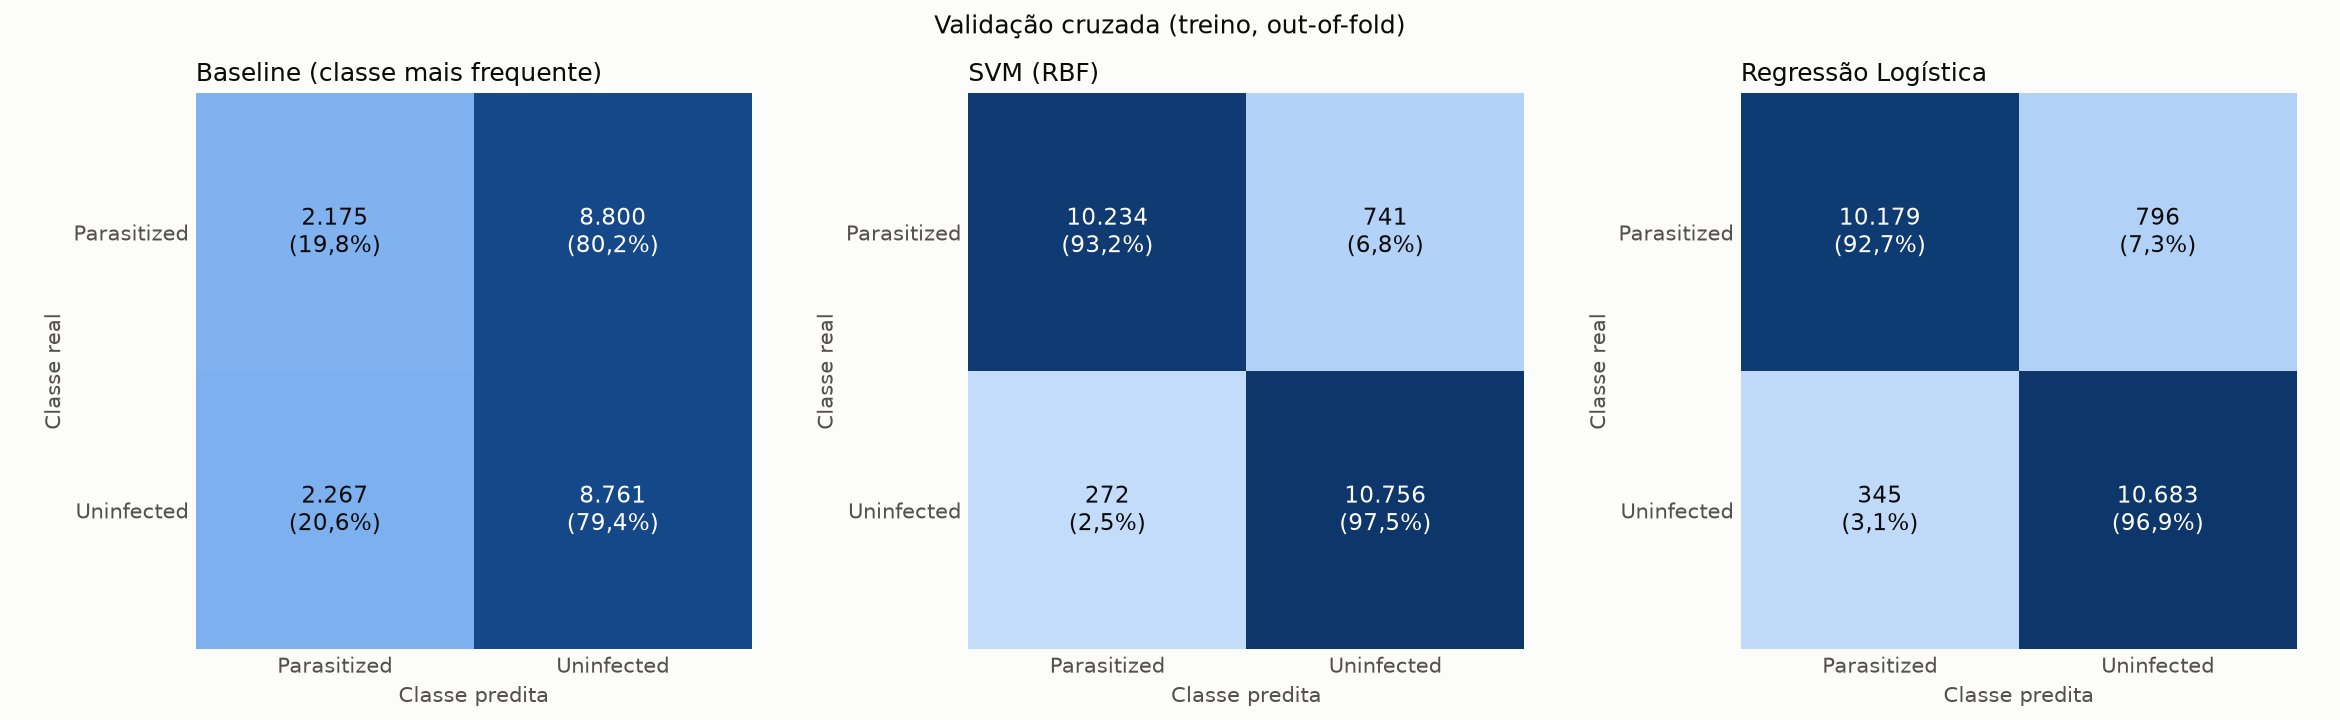
\includegraphics[width=\textwidth]{matrizes_confusao_cv.png}
\caption{Matrizes de confusão das predições fora da partição na validação cruzada (treino), com a
porcentagem de cada linha (classe real). Arquivo: \texttt{matrizes\_confusao\_cv.png}.}\label{fig:conf-cv}
\end{figure}

\begin{figure}[H]
\centering
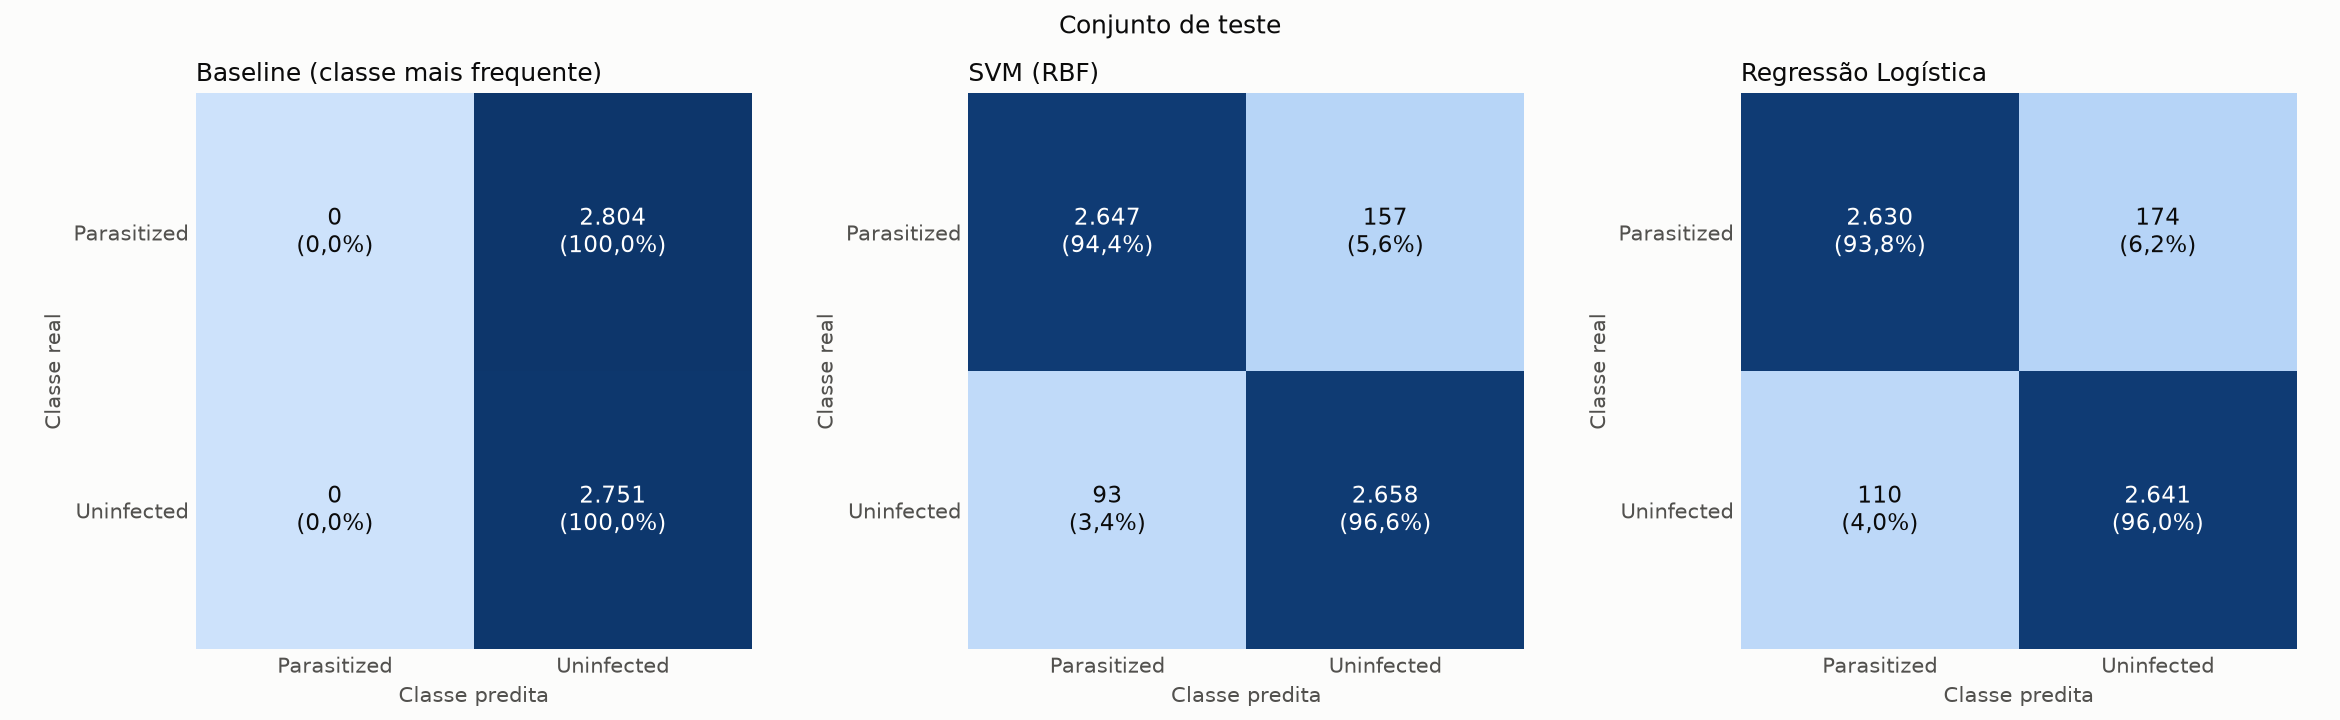
\includegraphics[width=\textwidth]{matrizes_confusao_teste.png}
\caption{Matrizes de confusão no conjunto de teste. Arquivo:
\texttt{matrizes\_confusao\_teste.png}.}\label{fig:conf-teste}
\end{figure}

\paragraph{Baseline.} No teste o baseline prevê sempre \textit{Uninfected} (a classe mais frequente
no treino) e acerta 49,5\% das imagens, com F1 macro de 0,331: F1 zero para as parasitadas e 0,662
para as não infectadas. Na validação cruzada o F1 macro calculado sobre as predições juntadas é maior
(0,448) porque a classe majoritária muda de uma partição para outra (as partições são formadas por
pacientes inteiros) e as predições juntadas acabam contendo as duas classes; a média do F1 de cada
partição, usada na busca, é 0,332. Em qualquer caso, os dois modelos ficam mais de 60 pontos de F1
acima da referência, o que mostra que as características carregam informação real sobre a classe.

\paragraph{Comparação entre os modelos.} O SVM é melhor que a regressão logística em todas as métricas,
mas por pouco (0,6 ponto de F1 macro no teste). As duas classes têm F1 praticamente igual. O tipo de
erro, porém, não é simétrico: os dois modelos têm recall menor para \textit{Parasitized} (0,944 no SVM)
que para \textit{Uninfected} (0,966). Ou seja, o erro mais comum é deixar passar uma célula
parasitada (157 falsos negativos contra 93 falsos positivos no SVM), que é o erro mais grave do ponto
de vista clínico. Os resultados de validação cruzada e de teste são muito próximos (0,954 e 0,955 no
SVM), o que indica que não houve sobreajuste na seleção de hiperparâmetros.

\subsection{Características: só cor vs. cor + textura}\label{sec:res-features}

Para avaliar a contribuição da textura, a configuração final foi repetida usando só as 61
características de cor (sem as 10 do LBP), com os mesmos dados, partições e grades.

\begin{table}[H]
\centering
\caption{Comparação entre conjuntos de características na configuração final (F1 macro).}\label{tab:features-res}
\begin{tabular}{lrcccc}
\toprule
& & \multicolumn{2}{c}{SVM (RBF)} & \multicolumn{2}{c}{Regressão logística} \\
\cmidrule(lr){3-4}\cmidrule(lr){5-6}
Conjunto & Qtd. & CV & Teste & CV & Teste \\
\midrule
Só cor           & 61 & 0,954 & 0,957 & 0,949 & 0,950 \\
Cor + textura    & 71 & 0,954 & 0,955 & 0,948 & 0,949 \\
\bottomrule
\end{tabular}
\fonte{outputs/64x64_normalizacao_cor_so_cor/ e outputs/64x64_normalizacao_cor/ (validacao_cruzada e testset/metricas_gerais.csv)}
\end{table}

As duas configurações empatam: a diferença na validação cruzada é de 0,0002 no SVM e de 0,001 na
regressão logística, muito abaixo do desvio entre partições. Depois da normalização de cor, a
textura medida pelo LBP não acrescenta informação às características de cor. Uma explicação plausível
é que o principal padrão local que o LBP detecta nestas imagens é o contraste do ponto escuro do
parasita, que os histogramas e desvios de cor já capturam. Numa verificação anterior, sem
normalização de cor, a combinação de momentos de cor com LBP tinha sido ligeiramente melhor que só os
momentos na regressão logística (0,923 contra 0,918), ou seja, a textura ajudava um pouco quando a
cor ainda carregava a variação entre lâminas.

A configuração final, definida antes desta comparação, mantém as 71 características. O resultado
indica que o LBP poderia ser removido sem perda, simplificando o modelo e a extração.

\subsection{Contribuição da segmentação}\label{sec:res-seg}

Para avaliar a segmentação, a configuração final foi repetida sem máscara: todas as estatísticas, a
normalização de cor e os histogramas passam a usar a imagem inteira, incluindo o fundo preto.

\begin{table}[H]
\centering
\caption{Contribuição da segmentação na configuração final (F1 macro).}\label{tab:seg-res}
\begin{tabular}{lcccc}
\toprule
& \multicolumn{2}{c}{SVM (RBF)} & \multicolumn{2}{c}{Regressão logística} \\
\cmidrule(lr){2-3}\cmidrule(lr){4-5}
Segmentação & CV & Teste & CV & Teste \\
\midrule
Sem (imagem inteira) & 0,947 & 0,950 & 0,937 & 0,947 \\
Com (máscara da célula) & 0,954 & 0,955 & 0,948 & 0,949 \\
\bottomrule
\end{tabular}
\fonte{outputs/64x64_normalizacao_cor_sem_segmentacao/ e outputs/64x64_normalizacao_cor/ (metricas_gerais.csv)}
\end{table}

A segmentação melhora o F1 macro de validação cruzada em 0,7 ponto no SVM e 1,1 ponto na regressão
logística; no teste, em 0,5 e 0,2 ponto. O ganho é modesto, da ordem do desvio entre partições, mas
aparece nos dois modelos e nas mesmas partições, então é consistente. Sem a máscara, cerca de 30\% dos
pixels são fundo preto: a média e o desvio de cada canal passam a depender de quanto fundo o recorte
tem (isto é, do formato da célula), os histogramas ganham um pico em zero e a normalização de cor
divide pela média da imagem inteira, que também depende da quantidade de fundo. O classificador ainda
funciona bem porque as faixas do histograma que contêm a célula continuam lá, mas misturadas a
informação de forma que não tem relação com o parasita.

\subsection{Análise dos erros}\label{sec:res-erros}

A análise usa as predições por imagem do conjunto de teste
(\arq{outputs/64x64_normalizacao_cor/testset/predicoes.csv}). A Figura~\ref{fig:erros} mostra
exemplos sorteados de erros do SVM.

\begin{figure}[H]
\centering
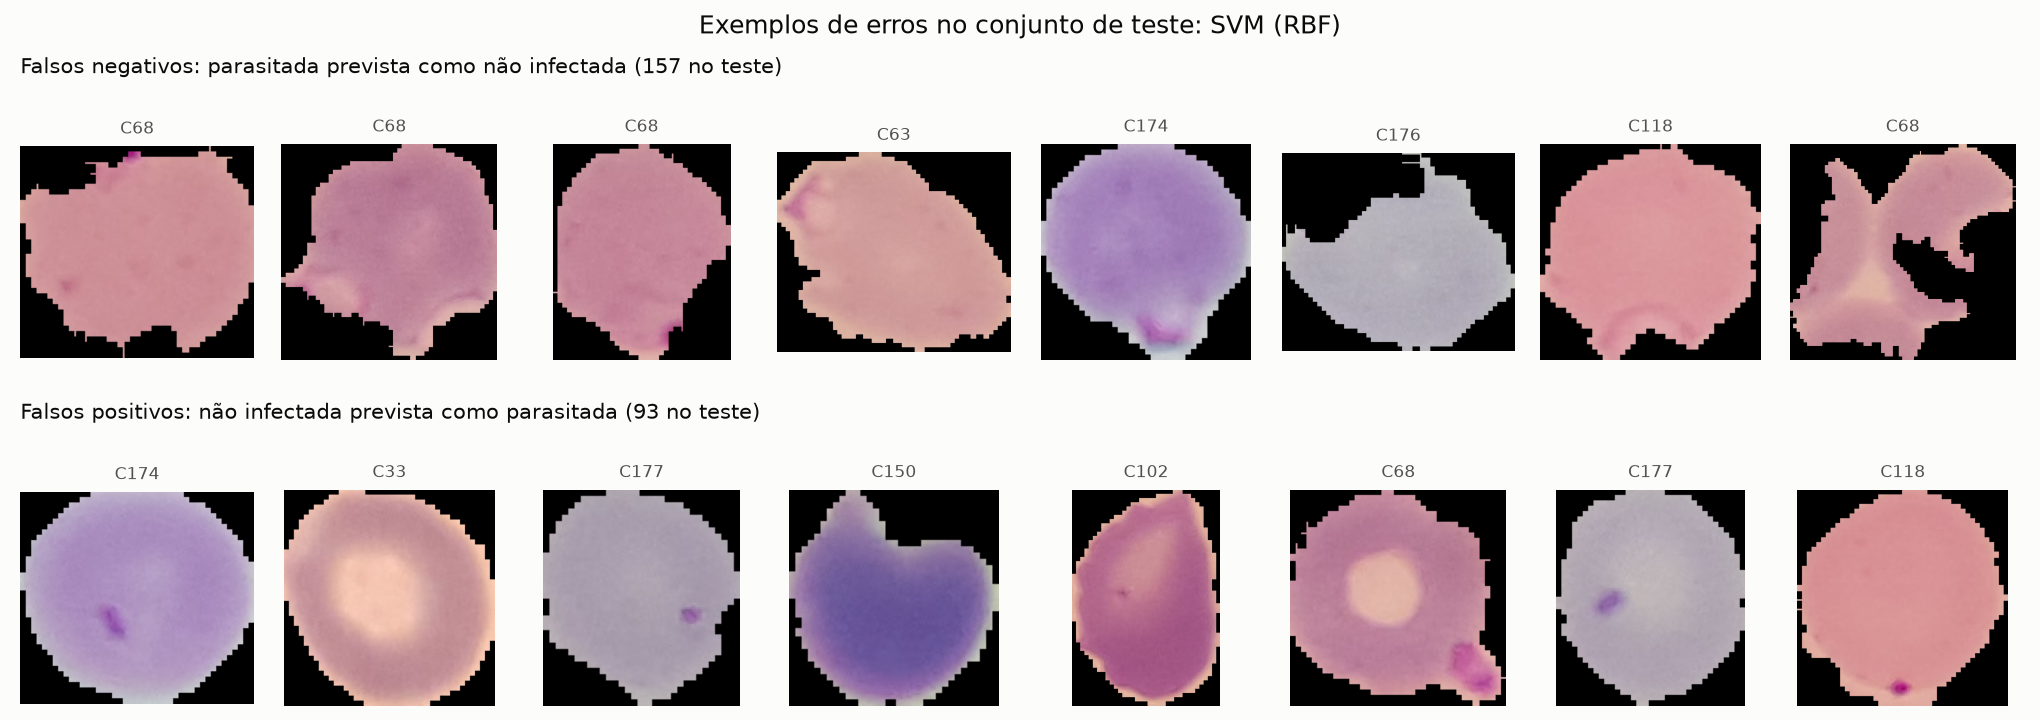
\includegraphics[width=\textwidth]{erros_exemplos.png}
\caption{Exemplos sorteados (semente 42) de erros do SVM no teste. Acima, falsos negativos
(parasitadas previstas como não infectadas); abaixo, falsos positivos. O título de cada imagem é o
paciente. Arquivo: \texttt{erros\_exemplos.png}.}\label{fig:erros}
\end{figure}

\paragraph{Quantidade e sobreposição.} O SVM erra 250 das 5.555 imagens de teste (157 falsos negativos
e 93 falsos positivos) e a regressão logística erra 284 (174 e 110). Dos 250 erros do SVM, 201 também
são erros da regressão logística: os erros vêm principalmente de imagens difíceis, e não de uma
fraqueza específica de um modelo.

\paragraph{Concentração por paciente.} Os erros não se distribuem de maneira uniforme entre os 40
pacientes de teste. A taxa de erro mediana por paciente é de 3,0\%, mas chega a 16,5\% (paciente
C102). Um único paciente, C68, concentra 59 erros (23,6\% do total), dos quais 56 são falsos
negativos entre suas 633 células parasitadas; os 5 pacientes com mais erros respondem por 47\% de
todos os erros e os 10 primeiros, por 66\%. Isso reforça que as características de cada lâmina
(coloração, estágio do parasita, qualidade da imagem) influenciam o resultado, mesmo após a
normalização de cor, e justifica a divisão por paciente: uma divisão aleatória por imagem teria
colocado células de C68 no treino e escondido essa dificuldade. A taxa de falsos positivos é de
4,3\% (32 de 748) nas células de pacientes saudáveis e de 3,0\% (61 de 2.003) nas células não
infectadas de pacientes infectados.

\paragraph{Inspeção visual.} Na Figura~\ref{fig:erros}:
\begin{itemize}
  \item \textbf{Falsos negativos}: o parasita é muito pequeno, pouco corado ou está na borda da célula
        (onde a erosão da máscara remove pixels e o LBP é contaminado pelo fundo). Em algumas imagens
        não se vê parasita algum na resolução da imagem, o que pode corresponder a formas muito jovens
        do parasita ou a erros de rótulo.
  \item \textbf{Falsos positivos}: várias células têm um ponto roxo nítido, semelhante a um parasita.
        Pode tratar-se de plaquetas ou resíduos de corante sobrepostos à célula, ou de erros de rótulo
        no próprio dataset; não é possível distinguir esses casos sem um especialista. Outros falsos
        positivos têm coloração muito escura ou saturada (por exemplo, a célula azul-escura do paciente
        C150) ou uma palidez central forte, casos que a normalização pela média não corrige
        totalmente.
\end{itemize}

%=====================================================================
\section{Discussão}\label{sec:discussao}
%=====================================================================

\paragraph{Quais decisões mais influenciaram o desempenho.} Ordenadas pelo efeito medido na validação
cruzada do SVM:
\begin{enumerate}
  \item \textbf{Normalização de cor por imagem}: cerca de +2 pontos de F1 macro no SVM e +3 na regressão
        logística (Tabela~\ref{tab:preproc}). A variação de coloração entre lâminas era a maior fonte de
        erro, como a análise de cor havia indicado (as cores mais frequentes são as mesmas nas duas
        classes e mudam de lâmina para lâmina).
  \item \textbf{Máscara correta}: calcular a máscara na resolução original e erodi-la, em vez de usar
        um limiar após o redimensionamento, rendeu +0,9 ponto (Tabela~\ref{tab:evolucao}).
  \item \textbf{Segmentação}: +0,7 ponto no SVM e +1,1 na regressão logística
        (Tabela~\ref{tab:seg-res}), por impedir que o fundo, cuja quantidade depende do formato do
        recorte, contamine as estatísticas e a normalização.
  \item \textbf{Textura (LBP)}: nenhum efeito mensurável depois da normalização de cor
        (Tabela~\ref{tab:features-res}); a informação útil já está nas características de cor.
  \item \textbf{Redimensionamento}: nenhum efeito mensurável entre 64x64, fator 2 e resolução original.
        A distorção de escala e de proporção do 64x64, que era uma preocupação teórica para o LBP, não
        se refletiu no resultado, e a resolução original não trouxe ganho apesar do detalhe extra.
\end{enumerate}

\paragraph{Quais características funcionaram melhor.} As características de \emph{distribuição} de cor
(histogramas, especialmente do canal G, e desvios padrão) são as mais informativas, porque capturam a
pequena região escura e roxa do parasita, que a média da célula praticamente não registra. Isso é
coerente com a análise de cor da Seção~\ref{sec:cor} e com a física do corante.

\paragraph{Quais classificadores funcionaram melhor.} O SVM com kernel RBF foi o melhor em todas as
configurações. A vantagem sobre a regressão logística, que era de quase 2 pontos sem normalização,
caiu para 0,6 ponto com normalização: depois de remover a coloração da lâmina, a fronteira entre as
classes no espaço de características fica quase linear. O desempenho do SVM é estável numa faixa
larga de hiperparâmetros (Tabela~\ref{tab:grid-svm}).

\paragraph{Classes confundidas e fatores que explicam os erros.} Com apenas duas classes, a confusão é
entre elas; o erro predominante é o falso negativo (parasitada classificada como não infectada). Os
fatores identificados na análise de erros são: (i) parasitas pequenos, pouco corados ou na borda da
célula; (ii) artefatos (plaquetas, resíduos de corante, palidez central) que imitam o parasita;
(iii) características próprias de algumas lâminas, que concentram os erros em poucos pacientes; e
(iv) possíveis erros de rótulo no dataset.

\paragraph{Limitações.}
\begin{itemize}
  \item O conjunto de teste tem 40 pacientes. Os erros se concentram em poucos deles, então a
        estimativa de desempenho no teste tem incerteza maior do que o número de imagens sugere;
        o desvio entre as partições da validação cruzada ($\sim$1 ponto de F1) dá uma ideia melhor
        dessa variabilidade. Diferenças menores que isso entre configurações não devem ser
        interpretadas como reais.
  \item Os histogramas de cor têm faixas sempre vazias e dependências lineares. Isso não prejudicou
        os modelos, mas um conjunto menor teria o mesmo desempenho.
  \item O LBP usa um único raio ($R=1$); Ojala et al.~\cite{ojala2002} recomendam combinar vários raios.
  \item Não foram usadas características de forma (área, perímetro, circularidade) nem de gradiente
        (HOG), sugeridas no enunciado como opções.
  \item A segmentação depende da segmentação original dos autores do dataset e herda seus defeitos.
\end{itemize}

\paragraph{Possíveis melhorias.} Ajustar o limiar de decisão para aumentar o recall de
\textit{Parasitized} (reduzindo falsos negativos à custa de mais falsos positivos), o que faz sentido
num contexto de triagem; normalizar a cor por lâmina (média de todas as células do mesmo paciente) em
vez de por imagem; usar LBP multiescala e características de coocorrência (GLCM); acrescentar a
assimetria (terceiro momento de cor), que deve captar a cauda escura do canal G; e revisar, com um
especialista, as imagens com suspeita de erro de rótulo.

%=====================================================================
\section{Conclusão}
%=====================================================================

Foi construído um pipeline completo de classificação de células de malária com características
extraídas manualmente e algoritmos tradicionais. A análise do dataset mostrou um problema
balanceado, sem imagens corrompidas nem duplicadas, com imagens de tamanhos variados e, sobretudo,
com grande variação de coloração entre lâminas. A divisão por paciente garantiu uma avaliação sem
vazamento.

Cada decisão do pipeline foi testada com experimentos controlados, escolhidos pela validação cruzada
e confirmados uma única vez no conjunto de teste. A normalização de cor por imagem foi a decisão de
maior impacto; a segmentação correta da célula também contribuiu, enquanto o redimensionamento não
teve efeito e foi mantido na forma mais simples. Duas falhas encontradas ao longo do caminho foram
corrigidas com base em verificação formal: a máscara contaminada pela borda e o tratamento linear de
uma variável circular (o matiz).

A configuração final (64x64, segmentação, normalização de cor, 71 características de cor e textura e
SVM com kernel RBF) obteve F1 macro de 0,955 e acurácia de 95,5\% no conjunto de teste, contra 0,331
de F1 macro do classificador de referência. O principal erro restante é deixar passar células
parasitadas com parasitas pequenos, pouco corados ou na borda, concentradas em poucos pacientes.

%=====================================================================
\appendix
\section{Reprodução e arquivos gerados}
%=====================================================================

Ambiente: Python 3.11, NumPy 2.4, pandas 3.0, scikit-learn 1.9, scikit-image 0.26, Pillow 12.3,
Matplotlib 3.11. Comandos, a partir da pasta \arq{AV2}:
\begin{itemize}
  \item \texttt{python 1\_analise\_dataset.py}: gera \arq{outputs/resumo.txt},
        \arq{outputs/cores_quantizadas.csv} e as Figuras~\ref{fig:balanceamento} a~\ref{fig:paleta};
  \item \texttt{python 2\_classificacao.py}: roda todas as configurações (as características são
        reaproveitadas dos CSV já existentes);
  \item \texttt{python 2\_classificacao.py <config> [...]}: roda só as configurações indicadas; a tabela
        \arq{outputs/comparacao_preprocessamento.csv} junta as métricas salvas de todas.
\end{itemize}

Estrutura de cada pasta \arq{outputs/<config>/}:
\begin{itemize}
  \item \arq{features_<config>.csv}: dataframe de características (as configurações
        \texttt{*\_so\_cor} reaproveitam o da configuração de origem);
  \item \arq{validacao_cruzada/}: \arq{grid_<modelo>.csv}, \arq{melhores_hiperparametros.csv},
        \arq{metricas_gerais.csv}, \arq{metricas_por_classe.csv} e \arq{matrizes_confusao_cv.png};
  \item \arq{testset/}: \arq{metricas_gerais.csv}, \arq{metricas_por_classe.csv},
        \arq{matrizes_confusao_teste.png}, \arq{predicoes.csv} (predição de cada modelo por imagem) e
        \arq{erros_exemplos.png}.
\end{itemize}
As pastas \arq{outputs/validacao_cruzada/} e \arq{outputs/testset/} (na raiz de \arq{outputs})
guardam a execução inicial (linha 1 da Tabela~\ref{tab:evolucao}).

\begin{thebibliography}{9}
\bibitem{rajaraman2018}
S.~Rajaraman, S.~K. Antani, M.~Poostchi, K.~Silamut, M.~A. Hossain, R.~J. Maude, S.~Jaeger e
G.~R. Thoma. Pre-trained convolutional neural networks as feature extractors toward improved malaria
parasite detection in thin blood smear images. \emph{PeerJ}, 6:e4568, 2018.

\bibitem{stricker1995}
M.~Stricker e M.~Orengo. Similarity of color images. In \emph{Storage and Retrieval for Image and
Video Databases III}, Proc. SPIE 2420, p.~381--392, 1995.

\bibitem{swain1991}
M.~J. Swain e D.~H. Ballard. Color indexing. \emph{International Journal of Computer Vision},
7(1):11--32, 1991.

\bibitem{ojala2002}
T.~Ojala, M.~Pietikäinen e T.~Mäenpää. Multiresolution gray-scale and rotation invariant texture
classification with local binary patterns. \emph{IEEE Transactions on Pattern Analysis and Machine
Intelligence}, 24(7):971--987, 2002.

\bibitem{mardia2000}
K.~V. Mardia e P.~E. Jupp. \emph{Directional Statistics}. Wiley, 2000.

\bibitem{buchsbaum1980}
G.~Buchsbaum. A spatial processor model for object colour perception. \emph{Journal of the Franklin
Institute}, 310(1):1--26, 1980.

\bibitem{sklearn}
F.~Pedregosa et al. Scikit-learn: machine learning in Python. \emph{Journal of Machine Learning
Research}, 12:2825--2830, 2011.

\bibitem{skimage}
S.~van der Walt et al. scikit-image: image processing in Python. \emph{PeerJ}, 2:e453, 2014.
\end{thebibliography}

\end{document}
